%%%%%%%%%%%%%%%%%%%%%%%%%%%%%%%%%%%%%%%%%%%%%%%%%%%%%%%%%%%%%%%%%%%%%%%%%%%%%%%%%%%%%%%%%%%%%%%%%%%%%%%%%%%%%%%%%%%%%%%%%%%%%%%%%%%%%%%%%%%%%%%%%%%%%%%%%%%%%%%%%%%%%%%%%%%%%%%%%%%%%%%%%%%%%%%%%%%%%%%%%%%%%%%%%%%%%%%%%%%%%%%%%%%%%%%%%%%
%%%%%%%%%%%%%%%%%%%%%%%%%%%%%%%%%%%%%%%%%%%%%%%%%%%%%%%%%%%%%%%%%%%%%%%%%%%%%%%%%%%%%%%%%%%%%%%%%%%%%%%%%%%%%%%%%%%%%%%%%%%%%%%%%%%%%%%%%%%%%%%%%%%%%%%%%%%%%%%%%%%%%%%%%%%%%%%%%%%%%%%%%%%%%%%%%%%%%%%%%%%%%%%%%%%%%%%%%%%%%%%%%%%%%%%%%%%
%%%%%%%%%%%%%%%%%%%%%%%%%%%%%%%%%%%%%%%%%%%%%%%%%%%%%%%%%%%%%%%%%%%%%%%%%%%%%%%%%%%%%%%%%%%%%%%%%%%%%%%%%%%%%%%%%%%%%%%%%%%%%%%%%%%%%%%%%%%%%%%%%%%%%%%%%%%%%%%%%%%%%%%%%%%%%%%%%%%%%%%%%%%%%%%%%%%%%%%%%%%%%%%%%%%%%%%%%%%%%%%%%%%%%%%%%%%
\chapter{Introduction}
\label{res:ch:Introduction}

The determination and quantification of the quality of the jet transverse momentum measurement is of crucial interest for many analyses with jet final states, \eg the measurement of the dijet cross section~\cite{bib:CMS:QCD_measurements} or \ttbar production cross sections~\cite{bib:CMS:TopCrossSection_8TeV}. 
Also searches for physics beyond the standard model with missing transverse momentum, \PTm, in the final state need a good knowledge of \PTm originating from wrongly measured jets~\cite{bib:CMS:RA2_8TeV,bib:CMS:MT2_8TeV,bib:CMS:AlphaT_8TeV}.
For analyses relying on information from simulation it is very important to correct the simulated resolution to the resolution actually present in data.
Therefore, scale factors will be presented to adjust the resolution in simulation to the resolution of the real detector.  
  
In the following sections, a data-based method to measure the jet \pt resolution in \GAMJET events will be presented. 
A similar method was already accomplished in earlier analyses~\cite{bib:CMS:JERCPaper_2011,bib:CMS-AN-2010-076,bib:CMS-AN-2010-141,bib:CMS-AN-2011-004} of 7\tev data.  
It is further developed here and applied to 8\tev data.

The method is based on the transverse momentum balance in the \GAMJET system. 
It takes advantage of the high resolution of the electromagnetic calorimeter and hence the excellent measurement of the photon energy and momentum.
Without initial and final state radiation, the photon and the jet are balanced in the transverse plane. 
Thus, measuring the photon \pt with high accuracy leads to an estimate of the true jet transverse momentum offering a possibility to quantify the resolution of jet \pt measurements.


%%%%%%%%%%%%%%%%%%%%%%%%%%%%%%%%%%%%%%%%%%%%%%%%%%%%%%%%%%%%%%%%%%%%%%%%%%%%%%%%%%%%%%%%%%%%%%%%%%%%%%%%%%%%%%%%%%%%%%%%%%%%%%%%%%%%%%%%%%%%%%%%%%%%%%%%%%%%%%%%%%%%%%%%%%%%%%%%%%%%%%%%%%%%%%%%%%%%%%%%%%%%%%%%%%%%%%%%%%%%%%%%%%%%%%%%%%%
%%%%%%%%%%%%%%%%%%%%%%%%%%%%%%%%%%%%%%%%%%%%%%%%%%%%%%%%%%%%%%%%%%%%%%%%%%%%%%%%%%%%%%%%%%%%%%%%%%%%%%%%%%%%%%%%%%%%%%%%%%%%%%%%%%%%%%%%%%%%%%%%%%%%%%%%%%%%%%%%%%%%%%%%%%%%%%%%%%%%%%%%%%%%%%%%%%%%%%%%%%%%%%%%%%%%%%%%%%%%%%%%%%%%%%%%%%%
%%%%%%%%%%%%%%%%%%%%%%%%%%%%%%%%%%%%%%%%%%%%%%%%%%%%%%%%%%%%%%%%%%%%%%%%%%%%%%%%%%%%%%%%%%%%%%%%%%%%%%%%%%%%%%%%%%%%%%%%%%%%%%%%%%%%%%%%%%%%%%%%%%%%%%%%%%%%%%%%%%%%%%%%%%%%%%%%%%%%%%%%%%%%%%%%%%%%%%%%%%%%%%%%%%%%%%%%%%%%%%%%%%%%%%%%%%%
\chapter{General approach of the resolution measurement using photon+jet events}
\label{res:ch:GeneralApproach}

The jet transverse momentum resolution is defined as the standard deviation of the jet transverse momentum response distribution with the response defined as the ratio of the reconstructed to the generator-level jet transverse momentum 
\begin{equation}\label{res:eq:responseFormula}
\mathcal{R} =  \frac{\pt^{\text{reco. jet}}}{\pt^{\text{gen. jet}}}.
\end{equation}
The transverse momentum of the generator-level jet is hereby defined as the sum of all particles' transverse momenta that are clustered into the jet cone.
It can differ to the momentum of the original final state quark or gluon by out-of-cone showering effects.
Out-of-cone showering refers to particles from the hadronisation process that are not clustered into the jet cone.
Throughout the following sections, the jet transverse momentum resolution will be abbreviated JER\footnote{This abbreviation is a historical relic from experiments where the momentum of jets were only measured in the calorimeters and therefore JER refered to jet energy resolution.}.

Figure~\ref{res:fig:TypicalResponse} shows a typical response distribution for jets in the barrel region.
\begin{figure}[b]
  \centering
      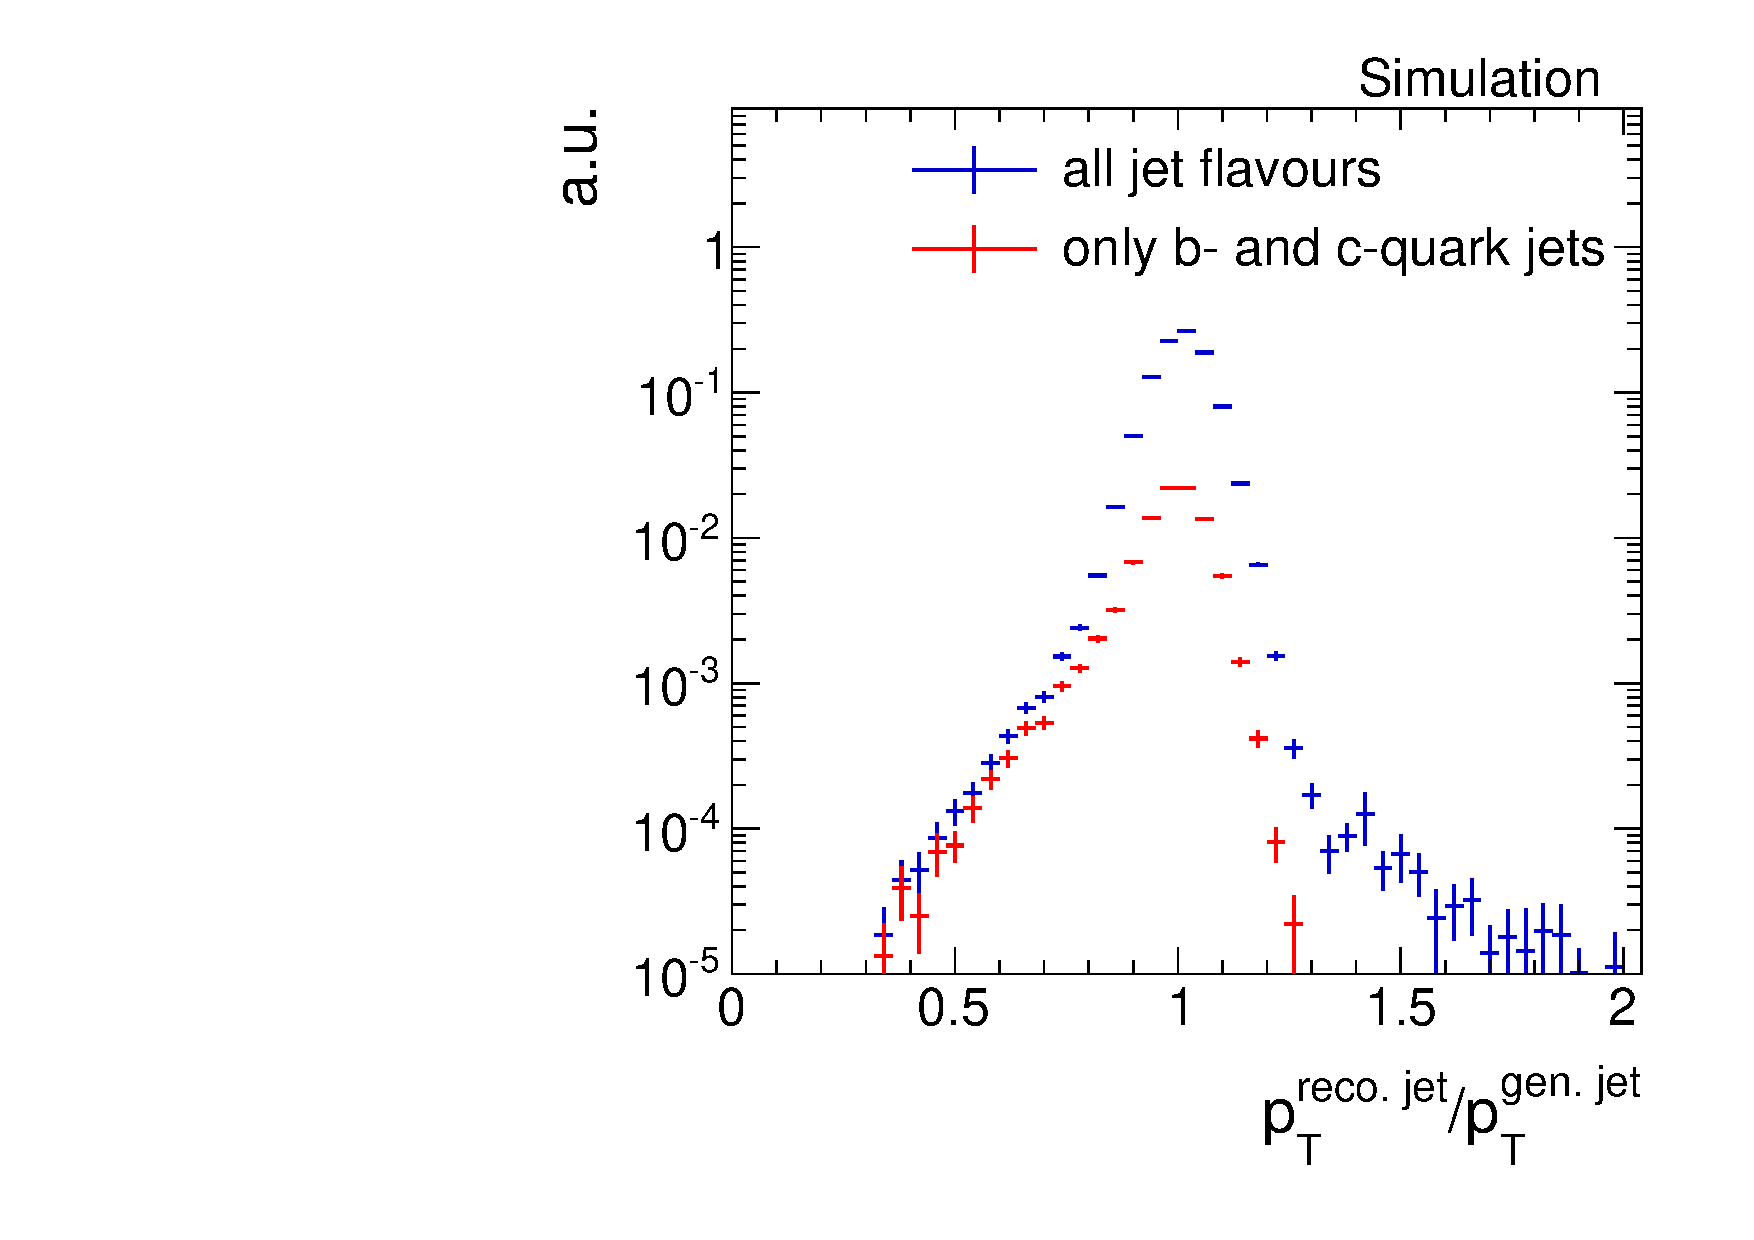
\includegraphics[width=0.49\textwidth]{figures/resolution/generalApproach/intrinsicExampleContributionofBCQuarks.pdf}
  \caption{Number of events over $\frac{\pt^{\text{reco. jet}}}{\pt^{\text{gen. jet}}}$ from a simulated \GAMJET sample. 
           The black dots show the contribution by c- and b-quark jets where the left tail originating from semi-leptonic decays of heavy quarks can be seen.}  
  \label{res:fig:TypicalResponse}
\end{figure}
The core of the response distribution shows a Gaussian behavior whereas the tails deviate from that functional form.
Physical reasons for the low response tail are inter alia semi-leptonic decays of heavy quarks where the neutrino cannot be detected and the reconstructed transverse momentum of the jet is too small (see Fig.~\ref{res:fig:TypicalResponse}). 
Only because neutrinos are included into the generator-level jet, this effect is visible.
Some instrumental effects, such as a non-linear response of the calorimeter, inhomogeneities of the detector material and electronic noise can contribute to both tails, 
others, like dead calorimeter channels only contribute to the left tail. 
The resolution is therefore determined using only the core of the distribution to avoid the coverage of non-Gaussian tails.
The resolution is thus defined as the standard deviation of the 99\% truncated response histogram devided by the mean of the histogram:

\begin{equation*}\label{res:eq:resolutionFormula}
\text{JER} = \frac{\sigma_{99\%}}{\mu_{99\%}}.
\end{equation*}

The determination of the 99\% range of the histogram is done in several steps. 
First the mean of the core is found via a Gaussian fit to the histogram in a 2$\sigma$ range\footnote{The 2$\sigma$ range is defined as the range [$\mu - 2\sigma$,$\mu + 2\sigma$].}. 
This procedure is done in three iteration steps.
Then, a symmetric interval around this mean is determined with its integral equal to 99\% of the integral of the full histogram. 

%The division by the mean is done to make the resolution measurement more insensitive to a variation of the jet energy scale (= mean of the response distribution)
%which has also an effect on the measured width of the distribution. 
%because response distributions with a scale smaller than one are typically narrower while distributions with scales larger than one are broader.

The evaluation of the response distribution as reconstructed over generated jet transverse momentum (Eq.~\eqref{res:eq:responseFormula})
is only possible for simulated events where generator-level information is accessible. 
A determination of the resolution in data, however, has to rely on a different approach.\\

The main idea of a resolution measurement using \GAMJET events is based on the transverse momentum balance of the \GAMJET system and the excellent electromagnetic calorimeter resolution
(which was estimated between 1.1 \% and 3.8\% in the barrel region for photons for $\sqrt{s}=8\tev$ data~\cite{bib:CMS:PhotonResolution_8TeV}).

In Fig~\ref{res:fig:FeynmanDiagrams}, all tree-level processes contributing to an event topology with one photon and one jet in the final state are depicted. 
\begin{figure}[b]
  \centering
      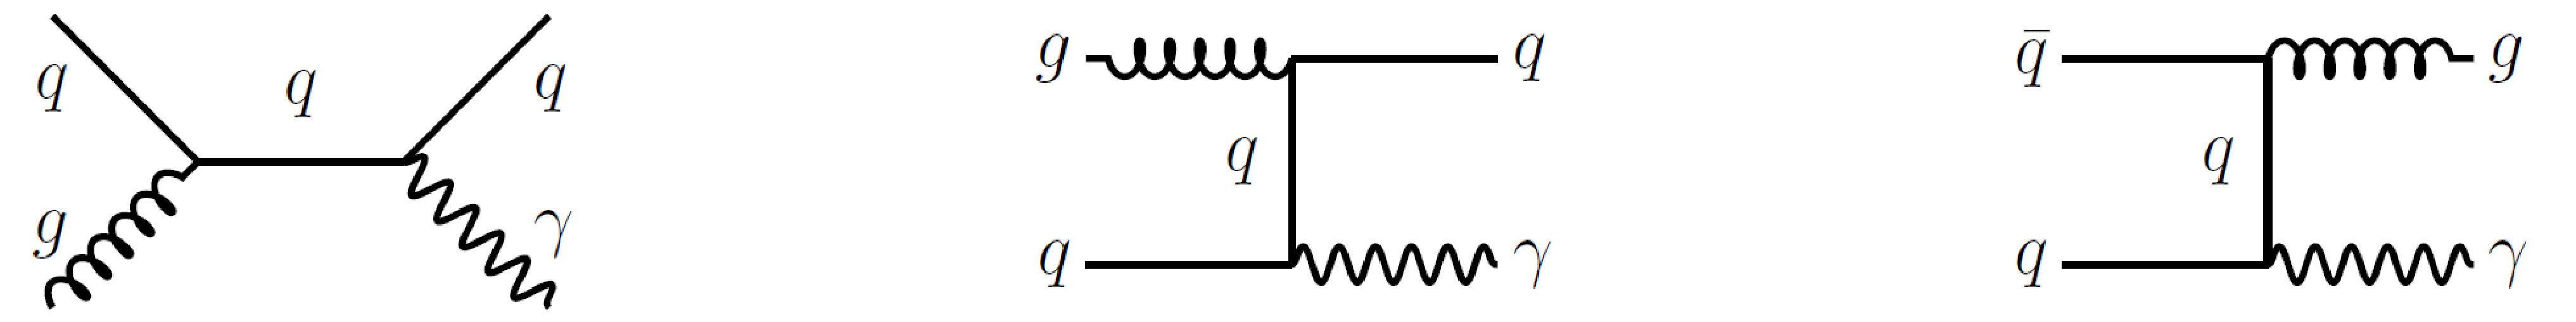
\includegraphics[width=0.99\textwidth]{figures/resolution/generalApproach/FeynmanDiagram.pdf}
  \caption{Tree-level Feynman diagrams of processes at the LHC in pp collisions with one photon and one jet in the final state.}  
  \label{res:fig:FeynmanDiagrams}
\end{figure}
Due to momentum conversation, the jet and the photon are back to back in the transverse plane, and therefore, $\ptvec^{\,\gamma} = -\ptvec^{\,\text{jet}}$. 
Because of the good resolution of the electromagnetic calorimeter, photon momenta can be very well measured 
and thus can serve as an excellent estimator for the true jet momentum.


Unfortunately, such clean events are very rare processes, and usually, the momentum balance is spoiled by initial and final state radiation, which lead to further jets in the event 
(see Fig.~\ref{res:fig:FeynmanDiagramsWithRadiation}). 
However, in order to select events that are balanced to a large extent, a lower bound 
on the angular distance in the transverse plane between the photon and the jet with the highest transverse momentum (leading jet) is required ($\Delta\Phi>2.95\,\unit{rad}$). 

Additionally, the variable 
\begin{equation*}\label{res:eq:alphaDef}
\alpha \doteq \frac{\pt^{\text{\nth{2} reco jet}}}{\pt^{\gamma}}
\end{equation*} 
is defined as a measure of further jet activity in an event. 
It is, however, not sufficient to require only an upper bound on $\alpha$. 
Instead, the jet energy resolution is measured in bins of $\alpha$ (with max($\alpha$) = 0.2), 
and the extrapolated value to zero further jet energy ($\alpha=0$) is taken as the measured resolution of the jet energy in the absence of further jets.
\begin{figure}[t]
  \centering
      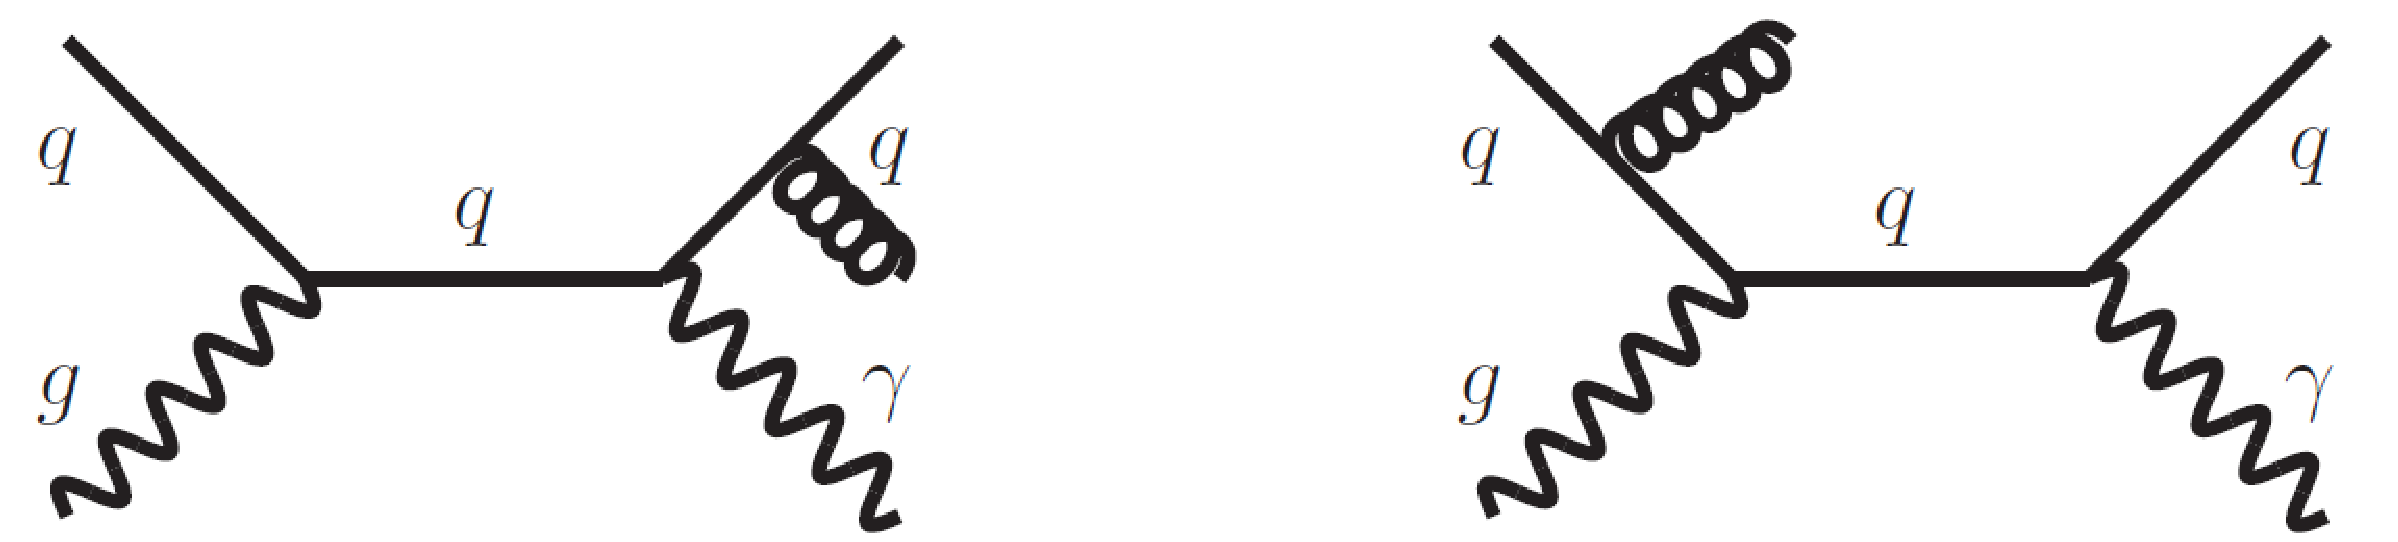
\includegraphics[width=0.60\textwidth]{figures/resolution/generalApproach/FeynmanDiagramsWithRadiation.pdf}
  \caption{Tree-level Feynman diagrams with initial and final state radiation.}  
  \label{res:fig:FeynmanDiagramsWithRadiation}
\end{figure}

Measuring the transverse momentum of the photon instead of taking the generator-level jet \pt leads to the fact that the measured resolution consists out of two parts
\begin{equation*}\label{res:eq:splitting}
\frac{\pt^{\text{reco. jet}}}{\pt^{\gamma}} = \underbrace{\frac{\pt^{\text{reco. jet}}}{\pt^{\text{gen. jet}}}}_{\text{intrinsic}} \cdot \underbrace{\frac{\pt^{\text{gen. jet}}}{\pt^{\gamma}}}_{\text{imbalance}}.
\end{equation*}
The intrinsic part is the resolution of interest which is independent of further jets in the event whereas the imbalance is strongly dependent on $\alpha$.

To extract the intrinsic resolution out of the measured one, the residual imbalance $q^{\prime}$ (the imbalance at $\alpha = 0$) is subtracted from the total resolution in the 
limit of vanishing additional jet activity. 
As that information is only available from simulation, the measured resolution in data is corrected by the residual imbalance taken from the simulated dataset.
%%%%%%%%%%%%%%%%%%%%%%%%%%%%%%%%%%%%%%%%%%%%%%%%%%%%%%%%%%%%%%%%%%%%%%%%%%%%%%%%%%%%%%%%%%%%%%%%%%%%%%%%%%%%%%%%%%%%%%%%%%%%%%%%%%%%%%%%%%%%%%%%%%%%%%%%%%%%%%%%%%%%%%%%%%%%%%%%%%%%%%%%%%%%%%%%%%%%%%%%%%%%%%%%%%%%%%%%%%%%%%%%%%%%%%%%%%%

%%%%%%%%%%%%%%%%%%%%%%%%%%%%%%%%%%%%%%%%%%%%%%%%%%%%%%%%%%%%%%%%%%%%%%%%%%%%%%%%%%%%%%%%%%%%%%%%%%%%%%%%%%%%%%%%%%%%%%%%%%%%%%%%%%%%%%%%%%%%%%%%%%%%%%%%%%%%%%%%%%%%%%%%%%%%%%%%%%%%%%%%%%%%%%%%%%%%%%%%%%%%%%%%%%%%%%%%%%%%%%%%%%%%%%%%%%%
%%%%%%%%%%%%%%%%%%%%%%%%%%%%%%%%%%%%%%%%%%%%%%%%%%%%%%%%%%%%%%%%%%%%%%%%%%%%%%%%%%%%%%%%%%%%%%%%%%%%%%%%%%%%%%%%%%%%%%%%%%%%%%%%%%%%%%%%%%%%%%%%%%%%%%%%%%%%%%%%%%%%%%%%%%%%%%%%%%%%%%%%%%%%%%%%%%%%%%%%%%%%%%%%%%%%%%%%%%%%%%%%%%%%%%%%%%%
\chapter{Datasets and event selection}

The measurement of the jet energy resolution is carried out with \GAMJET data recorded during the year 2012 at the CMS experiment.
The datasets and triggers that are exploitet for this measurement are introduced in the following Section~\ref{res:sec:DatasetsAndTriggers}.
In order to select \GAMJET events that are well suited for the resolution measurement, an event selection is applied on top. % to ensure \GAMJET events that show already the disired back-to-back signatures.
This event selection is described in Section~\ref{res:sec:EventSelection}.

\section{Datasets and triggers}
\label{res:sec:DatasetsAndTriggers}
This analysis exploits several triggers which were active during the year 2012 at the CMS experiment.
Because of the high production cross section of \GAMJET events, especially for low photon \pt, almost all of these triggers were highly prescaled, \ie only a fraction of events were actually recorded when the triggers fired.
All triggers that are utilised in this measurement are listed in Table~\ref{res:tab:triggers} together with their recorded luminosity.
\renewcommand{\arraystretch}{1.5}
\begin{table}[!hbt]
\centering
\caption{Single-photon triggers together with the recorded luminosity taking the prescales of the triggers into consideration.}
\label{res:tab:triggers}
\makebox[0.99\textwidth]{
\begin{tabular}{lr}
\multicolumn{2}{c}{} \\
\toprule
Trigger                       & Luminosity [\fbinv]   \\
\midrule
HLT\_Photon20\_CaloIdVL\_IsoL & 0.0008\\
HLT\_Photon30\_CaloIdVL\_IsoL & 0.0029\\
HLT\_Photon50\_CaloIdVL\_IsoL & 0.0607\\
HLT\_Photon75\_CaloIdVL\_IsoL & 0.123\\
HLT\_Photon90\_CaloIdVL\_IsoL & 0.373\\
HLT\_Photon135\               & 13.77\\
HLT\_Photon150\               & 19.71\\
\bottomrule
\multicolumn{2}{c}{} \\
\end{tabular}}
\end{table}  
The triggers rely on level one on single-photon triggers, such as L1SingleEG12 and L1SingleEG30.
The L1 triggers require at least one photon that is above a certain \pt threshold, \eg 12\gev or 30\gev.
The high-level triggers require a photon with a certain \pt (as indicated in the name) and, in case of thresholds below 135\gev also additional quality and isolation criteria. 
All triggers with threshold below 150\gev were prescaled.

The events that are selected by the above mentioned triggers are contained in the datasets listed in Table~\ref{res:tab:datasets}.
\renewcommand{\arraystretch}{1.5}
\begin{table}[!hbt]
\centering
\caption{Single-photon data samples used for the resolution measurement with the contained integrated luminosity.}
\label{res:tab:datasets}
\makebox[0.99\textwidth]{
\begin{tabular}{l r}
\multicolumn{2}{c}{} \\
\toprule
Dataset                                          & Luminosity [\fbinv]   \\
\midrule
 /Photon/Run2012A-22Jan2013-v1/AOD               &  0.876   \\
 /SinglePhoton/Run2012B-22Jan2013-v1/AOD         &  4.412  \\
 /SinglePhoton/Run2012C-22Jan2013-v1/AOD         &  7.055  \\
 /SinglePhotonParked/Run2012D-22Jan2013-v1/AOD   &  7.354  \\ 
\bottomrule
\multicolumn{2}{c}{} \\
\end{tabular}}
\end{table}  

\section{Simulated samples}
\label{res:sec:SimulatedSamples}

FIXME: What about QCD multijet sample -  maybe mentione here.
In order to compare the measured resolution in data to the resolution in simulation, a single-photon sample simulated with \pythiaSix is used.
This sample was generated flat in the photon \pt to have a good statistical precision also for the high photon \pt region.
In order to recover a physical \pt spectrum, all simulated events are reweighted.
Figure~\ref{res:fig:PhotonPtSpectrum} shows the photon \pt spectrum in simulation before and after the reweighting. 

All simulated samples come with a pileup scenario which does not necessarily match the pileup scenario in data. 
To match the measured distribution of primary vertices, the events are weighted according to their number of primary vertices. 
Because almost all of the used triggers are differently prescaled, the distributions of primary vertices differ among the various events triggered by the corresponding trigger.
Thus the reweighing has to be done separately for the events falling in the photon \pt range of the several triggers (see Table~\ref{res:tab:PhotonPtBins}).
A comparison between the number of primary vertices can be found in Appendix~\ref{res:app:pileup} for all triggers.
\begin{figure}[h]
  \centering
      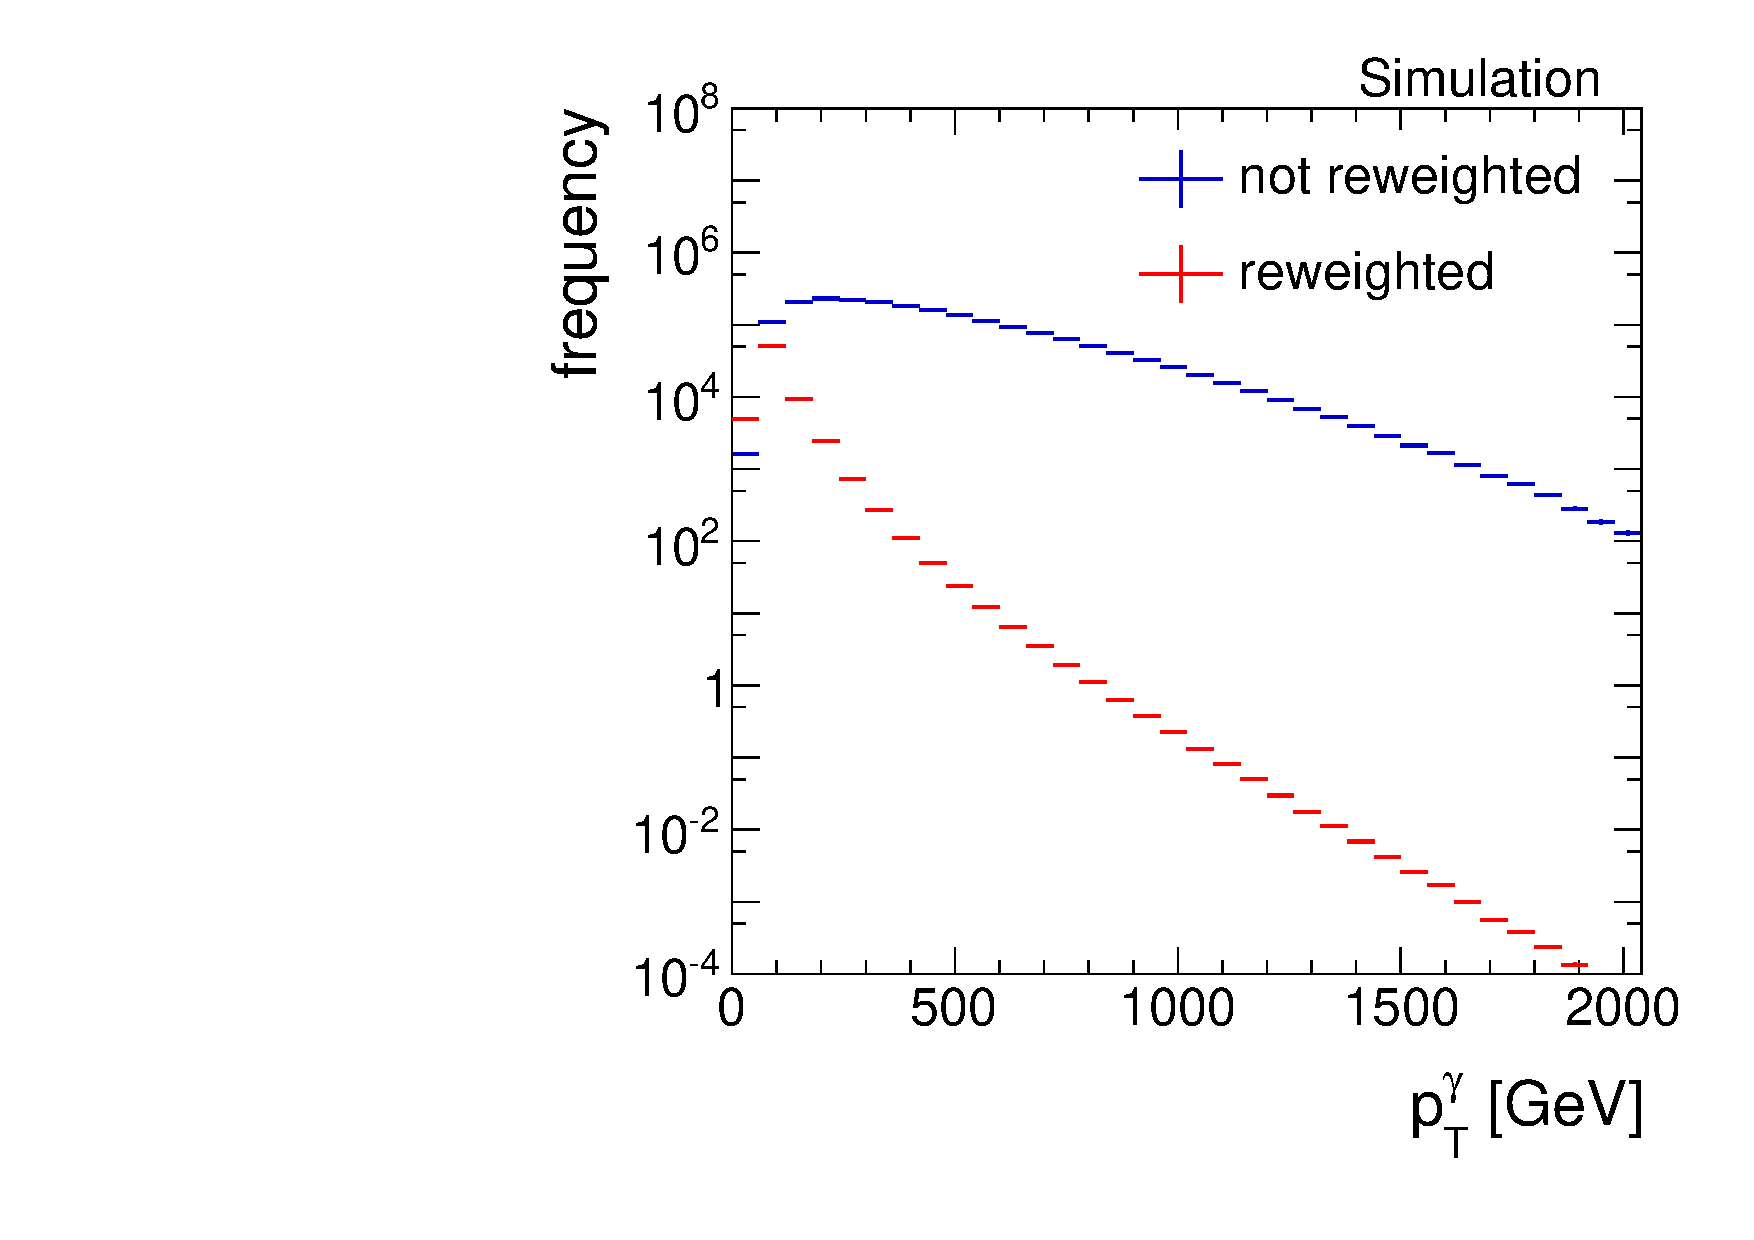
\includegraphics[width=0.49\textwidth]{figures/resolution/eventSelection/PhotonPtComparison_reweighted.pdf} 
  \caption{The photon \pt spectrum before (blue) and after (red) reweighing.}  
  \label{res:fig:PhotonPtSpectrum}
\end{figure}


\section{Event selection}
\label{res:sec:EventSelection}
Events are reconstructed with the particle-flow reconstruction algorithm, which uses information of all detector components to reconstruct individual particles~\cite{CMS-PAS-PFT-09-001}.
Furthermore, particles belonging to a jet are clustered with the Anti-k$_{\text{t}}$ jet clustering algorithm with a radius of R=0.5~\cite{Cacciari:2008gp}.

To select clean \GAMJET events, it is required that the leading jet meets the following requirements (these criteria correspond to a 'tight ID' in~\cite{website:JetIdentification,bib:CMS-AN-2010-003}):
\begin{itemize}

 \item Neutral hadron fraction $<$ 0.90
 \item Neutral electromagnetic fraction $<$ 0.90
 \item Number of constituents $>$ 1
\end{itemize}

 And for jets in the pseudorapidity range $|\eta^{\text{jet}}| < 2.4 $ :
\begin{itemize}
 \item Charged hadron fraction $>$ 0
 \item Charged hadron multiplicity $>$ 0
 \item Charged electromagnetic fraction $<$ 0.99
\end{itemize}
To mitigate effects from pileup, the first and second jet are required to have a transverse momentum greater 10\gev.

Concerning the photon, a maximal pseudorapidity of the photon of $|\eta^{\gamma}| < 1.3$ is demanded to exploit the high resolution of the ECAL in the barrel region.

Furthermore, the resolution is determined for different ranges in photon \pt to avoid mixing of different prescales of the various triggers. 
In Table~\ref{res:tab:PhotonPtBins} the applied binning is shown with the respective triggers contributing to each $\pt^{\gamma}$ bin.


\renewcommand{\arraystretch}{1.5}
\begin{table}[htb]
\centering
\caption{Photon \pt bins and corresponding triggers.}
\label{res:tab:PhotonPtBins}
\makebox[0.99\textwidth]{
\begin{tabular}{lc}
\multicolumn{2}{c}{} \\
\toprule
$\pt^{\gamma}$-bins           & Trigger         \\
\midrule
22\gev    & HLT\_Photon20\_CaloIdVL\_IsoL\_v* \\
36\gev    & HLT\_Photon30\_CaloIdVL\_IsoL\_v* \\
60\gev    & HLT\_Photon50\_CaloIdVL\_IsoL\_v* \\
88\gev    & HLT\_Photon75\_CaloIdVL\_IsoL\_v* \\
105\gev   & HLT\_Photon90\_CaloIdVL\_IsoL\_v* \\
149\gev   & HLT\_Photon135\_v*                \\
165\gev   & HLT\_Photon150\_v*                \\
\bottomrule
\multicolumn{2}{c}{} \\
\end{tabular}}
\end{table}

QCD multijets events constitute an important background to the \GAMJET events: A photon can be faked by a $\pi^{0}$ decaying into two close-by photons. 
Therefore, a very clean selection of the photons is necessary to suppress this background.
The following variables are used (see~\cite{CMS-PAS-EGM-10-006} for further explanation of the variables):

\begin{itemize}
 \item $\frac{\textbf{H}}{\textbf{E}}$ : The ratio of the measured energy in the hadronic calorimeter over the energy measured in the electromagnetic calorimeter. 
                                                    For photons, this is supposed to be very small as they deposit their energy predominantly in the ECAL.
 \item $\mathbold{\sigma_{i\eta i \eta}}$: The energy weighted spatial width of the photon energy deposition. The electromagnetic shower of a photon has a small lateral size 
                                           resulting in small $\sigma_{i\eta i \eta}$ for prompt photons while showers from fake photons, \eg $\pi^{0} \rightarrow \gamma \gamma$
                                           have a larger lateral size.
 \item \textbf{Jurassic ECAL isolation}: This isolation criterion uses the information of reconstructed hits ``RecHits'' (coming from the local reconstruction of the digital signals) 
                                         in a cone around the photon supercluster of R=0.4. Those are summed up and an upper criterion is identified to discriminate against 
                                         background which is typically spatially broader.  
 \item \textbf{Tower-based HCAL isolation}: The isolation criterion requires the energy deposited in all HCAL towers around the photon in cone of R=0.4 to be small compared to the 
                                            photon's energy. 
 \item \textbf{Hollow cone track isolation}: Requires absence of high-energetic tracks around the photon.
 \item \textbf{Pixel seed veto}: In order to reduce the background from electrons and positrons, the absence of a pixel-seed in the pixel tracker along the photons 
                                 trajectory is required.
\end{itemize}

The upper and lower bounds that are set on these observables can be found in Table~\ref{res:tab:PhotonIsolation}. 
\renewcommand{\arraystretch}{1.5}
\begin{table}[htb]
\centering
\caption{Upper and lower bounds for all photon isolation criteria in the barrel $\left( |\eta^{\gamma}|<1.4442 \right)$.}
\label{res:tab:PhotonIsolation}
\makebox[0.99\textwidth]{
\begin{tabular}{lc}
\multicolumn{2}{c}{} \\
\toprule
                              & Barrel                          \\
\midrule
$\frac{\text{H}}{\text{E}}$   & $<$ 0.05                        \\
$\sigma_{i\eta i \eta}$           & $<$ 0.013                       \\
ECAL isolation                & $<4.2 + 0.0060 \cdot \pt^{\gamma}$   \\
HCAL isolation                & $<2.2 + 0.0025 \cdot \pt^{\gamma}$   \\
Track Isolation               & $<2.0 + 0.0010 \cdot \pt^{\gamma}$   \\
Pixel seed veto               & yes                              \\
\bottomrule
\multicolumn{2}{c}{} \\
\end{tabular}}
\end{table}
%\begin{table}[bt]
%\caption{Upper and lower bounds for all photon isolation criteria in the barrel $\left( |\eta^{\gamma}|<1.4442 \right)$ and endcap $\left(1.4442 <|\eta^{\gamma}|<2.5 \right)$ .}
%\renewcommand{\arraystretch}{1.5}
%\begin{center}
%\begin{tabular}{ l| c | c |}
%                              & Barrel                                  & Endcap                                  \\\hline
%$\frac{\text{H}}{\text{E}}$   & $<$ 0.05                                & $<$ 0.05                                \\\hline
%$\sigma_{i\eta i \eta}$       & $<$ 0.013                               & $<$ 0.03                                \\\hline
%ECAL isolation                & $<4.2 + 0.0060 \, \pt^{\gamma}$   & $<4.2 + 0.0060 \, \pt^{\gamma}$    \\\hline
%HCAL isolation                & $<2.2 + 0.0025 \, \pt^{\gamma}$   & $<2.2 + 0.0025 \, \pt^{\gamma}$   \\\hline
%Track Isolation               & $<2.0 + 0.0010 \, \pt^{\gamma}$   & $<2.0 + 0.0010 \, \pt^{\gamma}$    \\\hline
%Pixel seed veto               & yes                                     & yes                                     \\\hline
%\end{tabular}
%\end{center}
%\label{tab:PhotonIsolation}
%\end{table}


Besides the mentioned requirements concerning the objects' attributes, two further criteria related to the event topology are crucial for this analysis:\\
An upper threshold on $\Delta \Phi$ between the leading jet and the photon and a maximal value for $\alpha$
\begin{itemize}
 \item $\Delta \Phi \left(\text{1st jet}, \gamma \right) > 2.95\,\unit{rad}$
 \item $\frac{\pt^{\text{2nd jet}}}{\pt^{\gamma}} < 0.20$.
\end{itemize}
These requirements are important to suppress events with too much further hadronic activity.

A summary of all selection criteria can be found in Appendix~\ref{res:app:eventselection}.
%%%%%%%%%%%%%%%%%%%%%%%%%%%%%%%%%%%%%%%%%%%%%%%%%%%%%%%%%%%%%%%%%%%%%%%%%%%%%%%%%%%%%%%%%%%%%%%%%%%%%%%%%%%%%%%%%%%%%%%%%%%%%%%%%%%%%%%%%%%%%%%%%%%%%%%%%%%%%%%%%%%%%%%%%%%%%%%%%%%%%%%%%%%%%%%%%%%%%%%%%%%%%%%%%%%%%%%%%%%%%%%%%%%%%%%%%%%

%%%%%%%%%%%%%%%%%%%%%%%%%%%%%%%%%%%%%%%%%%%%%%%%%%%%%%%%%%%%%%%%%%%%%%%%%%%%%%%%%%%%%%%%%%%%%%%%%%%%%%%%%%%%%%%%%%%%%%%%%%%%%%%%%%%%%%%%%%%%%%%%%%%%%%%%%%%%%%%%%%%%%%%%%%%%%%%%%%%%%%%%%%%%%%%%%%%%%%%%%%%%%%%%%%%%%%%%%%%%%%%%%%%%%%%%%%%
%%%%%%%%%%%%%%%%%%%%%%%%%%%%%%%%%%%%%%%%%%%%%%%%%%%%%%%%%%%%%%%%%%%%%%%%%%%%%%%%%%%%%%%%%%%%%%%%%%%%%%%%%%%%%%%%%%%%%%%%%%%%%%%%%%%%%%%%%%%%%%%%%%%%%%%%%%%%%%%%%%%%%%%%%%%%%%%%%%%%%%%%%%%%%%%%%%%%%%%%%%%%%%%%%%%%%%%%%%%%%%%%%%%%%%%%%%%
\chapter{Methodology of the measurement}

\interfootnotelinepenalty=10000

The basic methodology of exploiting the \pt balance in $\GAMJET$ events to measure the resolution and to extrapolate the result to small $\alpha$ has already been described
\mbox{in \cite{CMS-AN-2010-076}}. 
Here, the method is extended to explicitly distinguish the case of parton radiation in different event hemispheres.
For the sake of completeness, the full methodology will be explained.

As already described in Section \ref{sec:approach}, the idea behind a resolution measurement with $\GAMJET$ events is the usage of the photon energy instead of the true jet energy.
This results in a twofold contribution to the measured response, the intrinsic response and the imbalance:

\begin{equation}\label{eq:splittedResolution}
\frac{\pt^{\text{reco. jet}}}{\pt^{\gamma}} = \underbrace{\frac{\pt^{\text{reco. jet}}}{\pt^{\text{gen. jet}}}}_{\text{intrinsic}} \cdot \underbrace{\frac{\pt^{\text{gen. jet}}}{\pt^{\gamma}}}_{\text{imbalance}}.
\end{equation}

Taking the photon \pt as true jet \pt estimator instead of the generator jet \pt, and thus measuring the response defined as 
$\frac{\pt^{\text{reco. jet}}}{\pt^{\gamma}}$, results in a different shape
of the response function as shown in \mbox{Fig. \ref{fig:responseExamples}}. It compares the intrinsic response, the imbalance, and the measured total response in simulation. 

\begin{figure}[t]
 \centering
     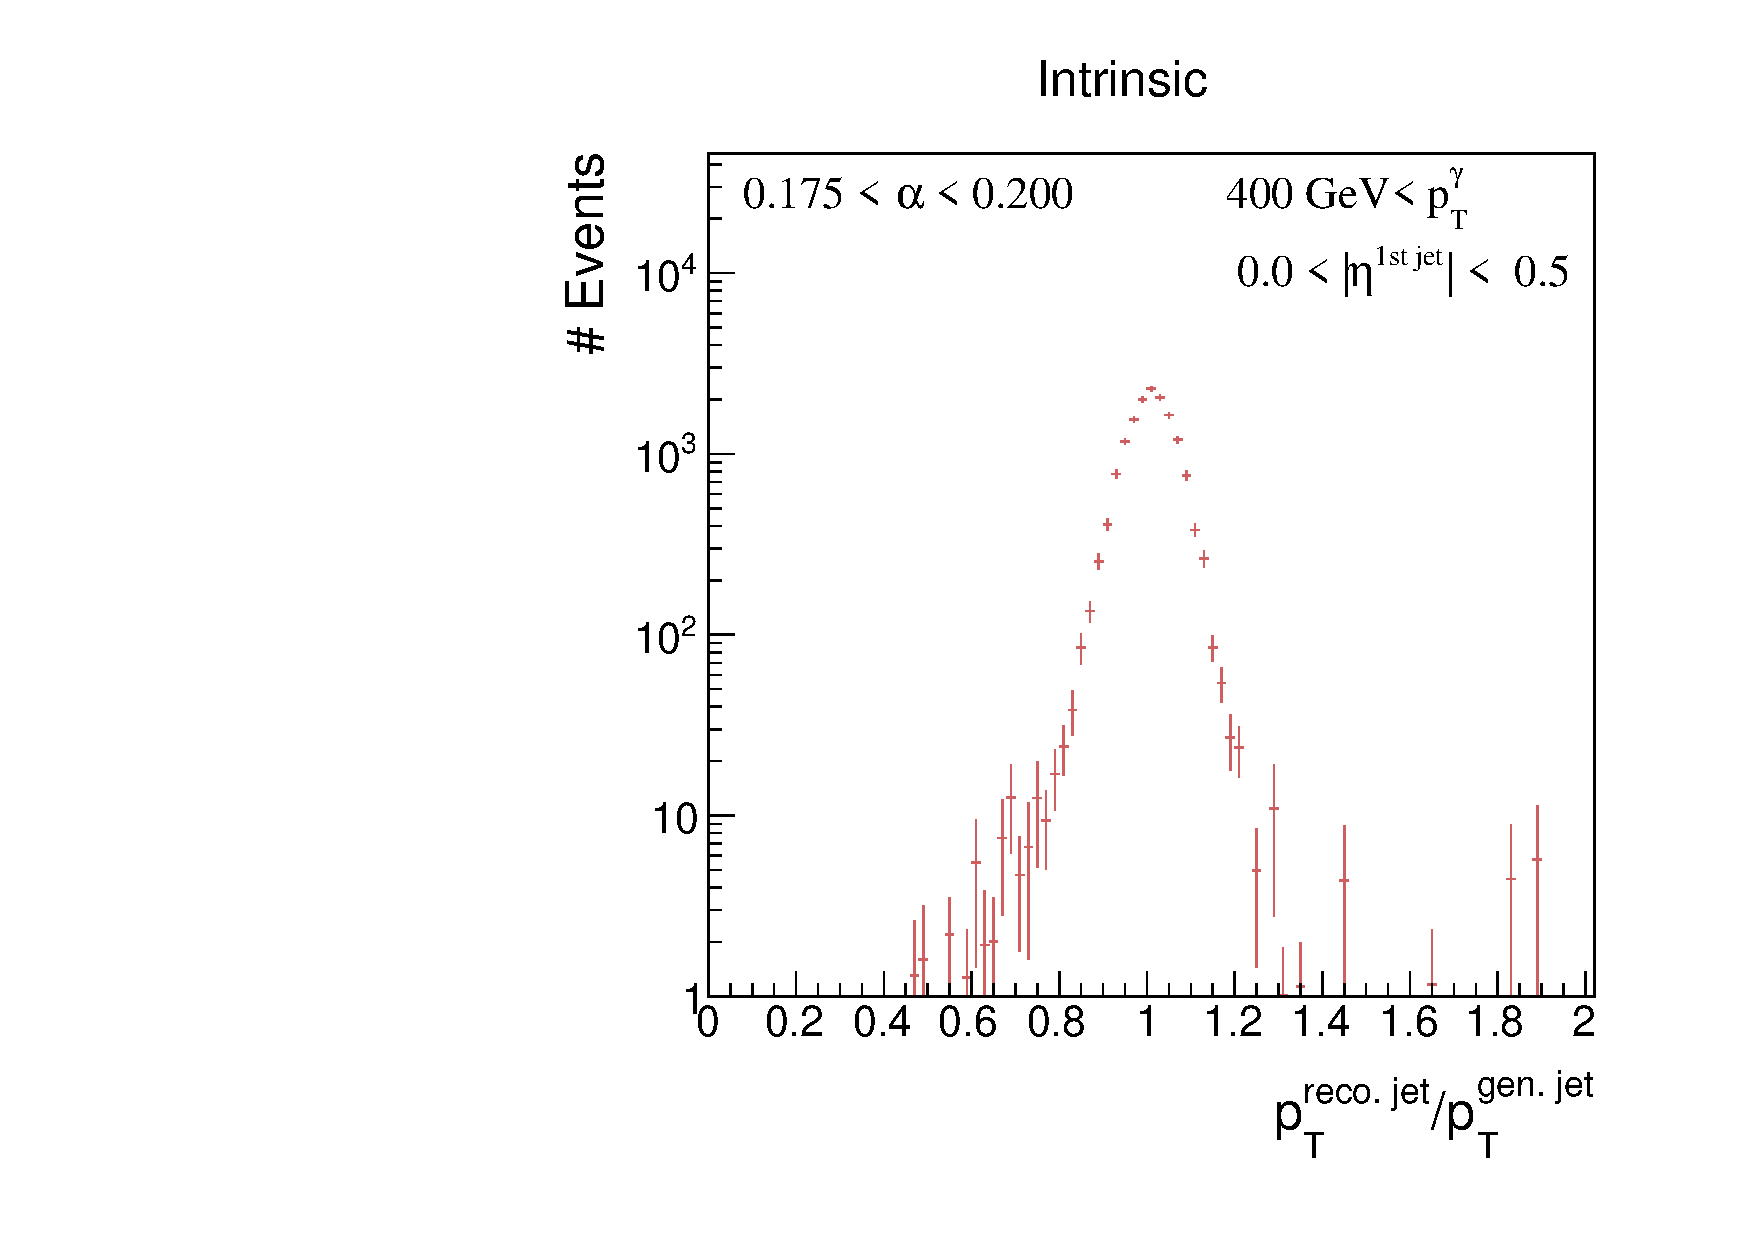
\includegraphics[width=0.49\textwidth]{figures/resolution/methodology/intrinsicExample.pdf}
     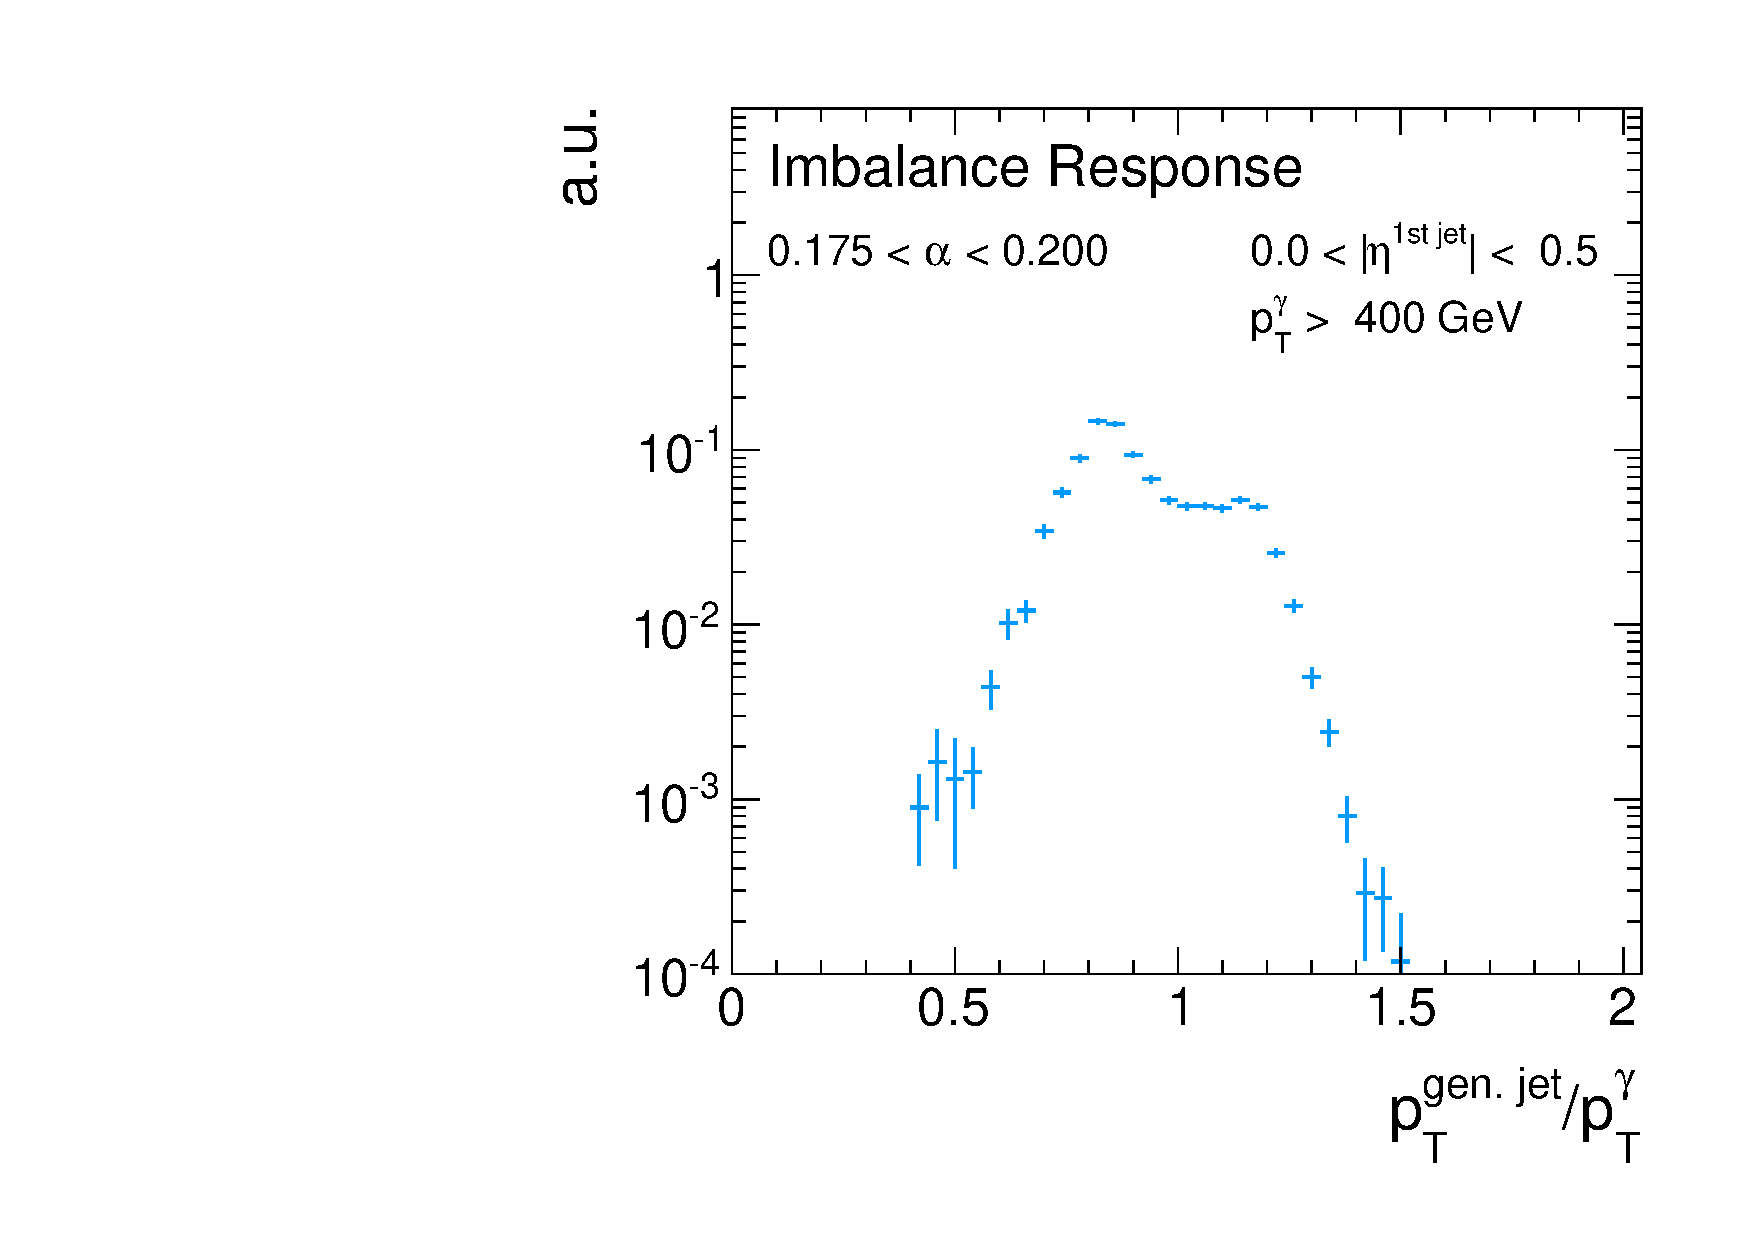
\includegraphics[width=0.49\textwidth]{figures/resolution/methodology/imbalanceExample.pdf}

     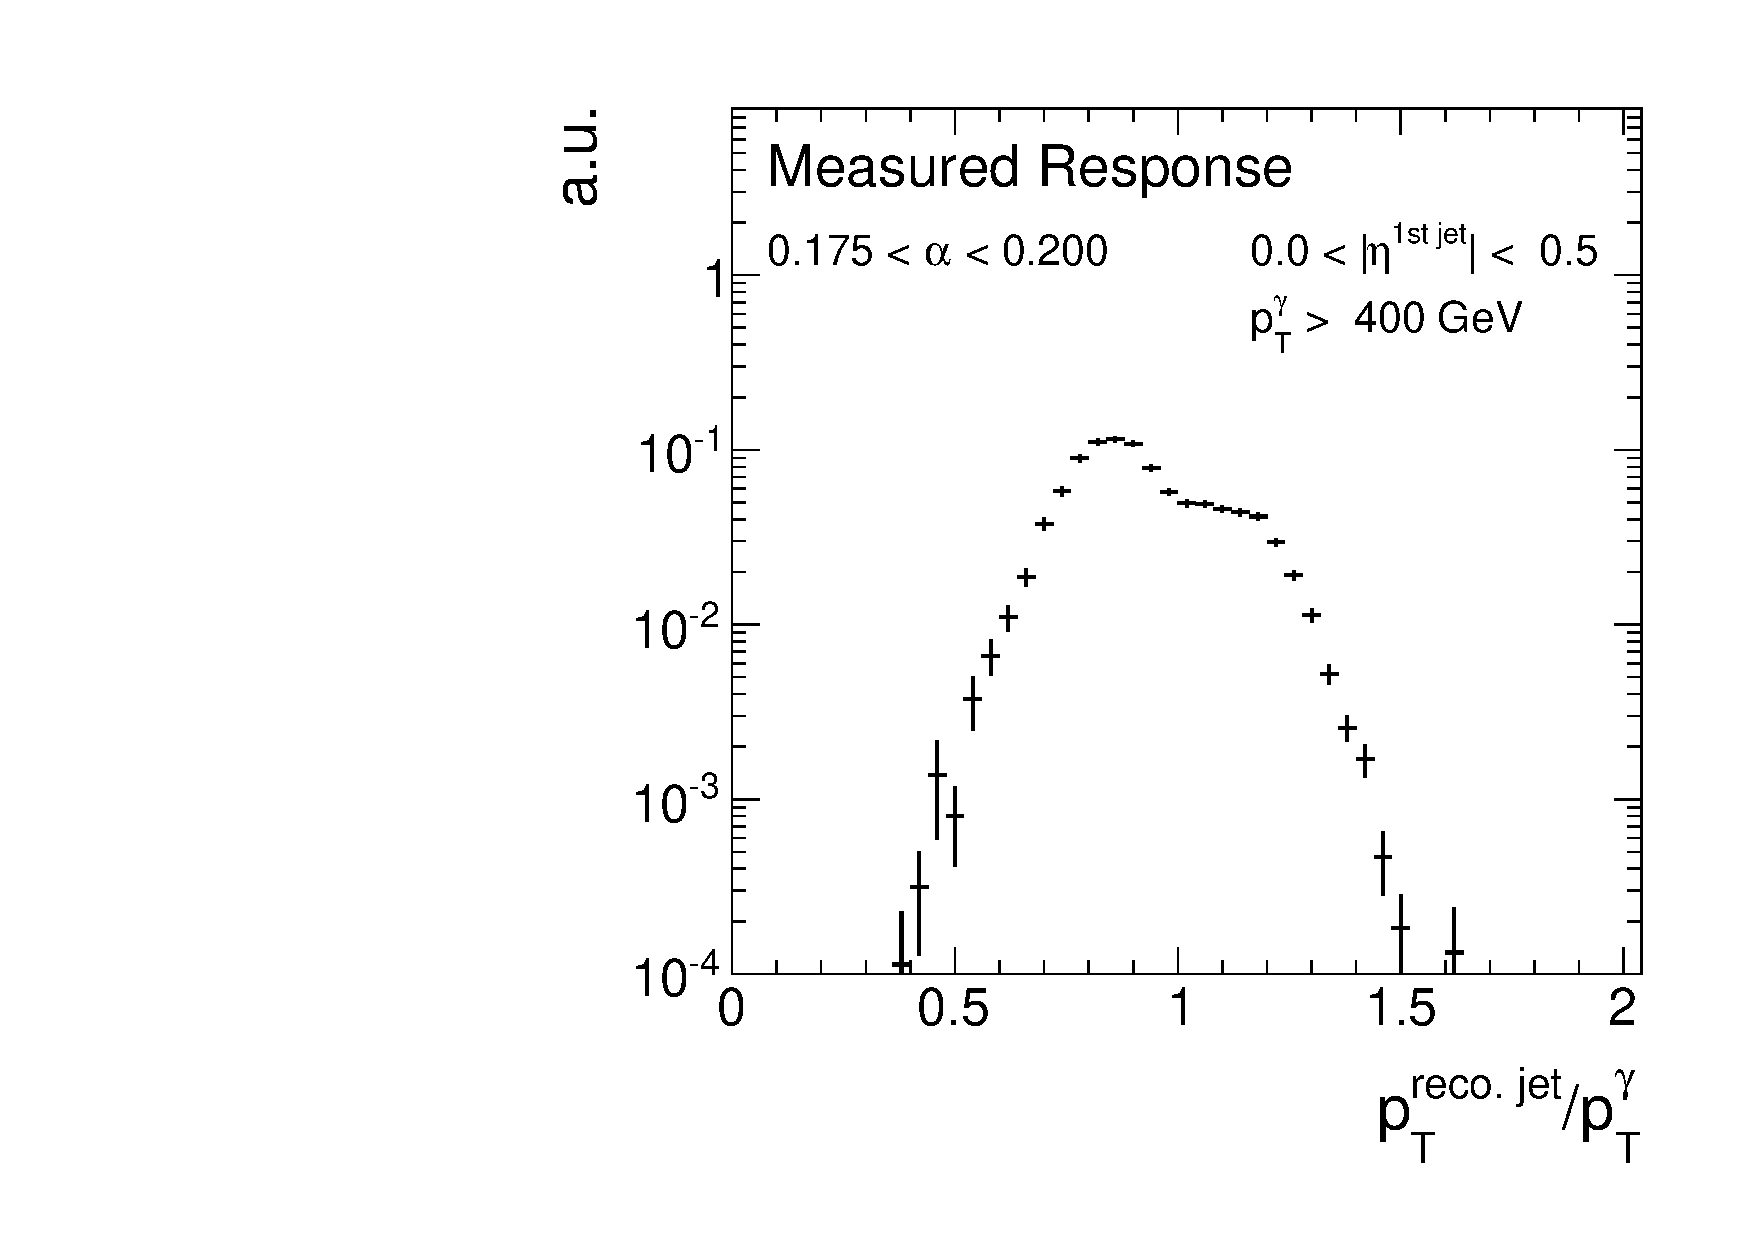
\includegraphics[width=0.49\textwidth]{figures/resolution/methodology/fullResponseExample.pdf}
  \caption{The two different contributions, intrinsic (top left) and imbalance (top right), to the measured response (bottom), 
           cf. \mbox{Eq.~\eqref{eq:splittedResolution}}, in simulated events.}  
 \label{fig:responseExamples}
\end{figure}


The clear difference between the intrinsic response and the imbalance is the double peak structure of the latter one. The measured response is a convolution of the two
contributions, where the double peak is consequentially less pronounced.

The occurrence of two peaks is caused by the hard selection in $\Delta \phi$ which forces the second jet to be either close to the photon or close to the leading jet 
due to \pt conservation. 
The possibility of an energetic second jet perpendicular to the leading jet photon axis which is balanced by a third jet is very unlikely 
due to the decreasing jet multiplicity in QCD events.
The double peak structure is less pronounced for small second jet \pt (small $\alpha$) where the $\Delta \Phi$ requirement does not have such a strong effect in rejecting
events with a second jet perpendicular to the photon leading jet axis (see \mbox{Fig. \ref{fig:alphaBins}}).

\begin{figure}[bt]
 \centering
     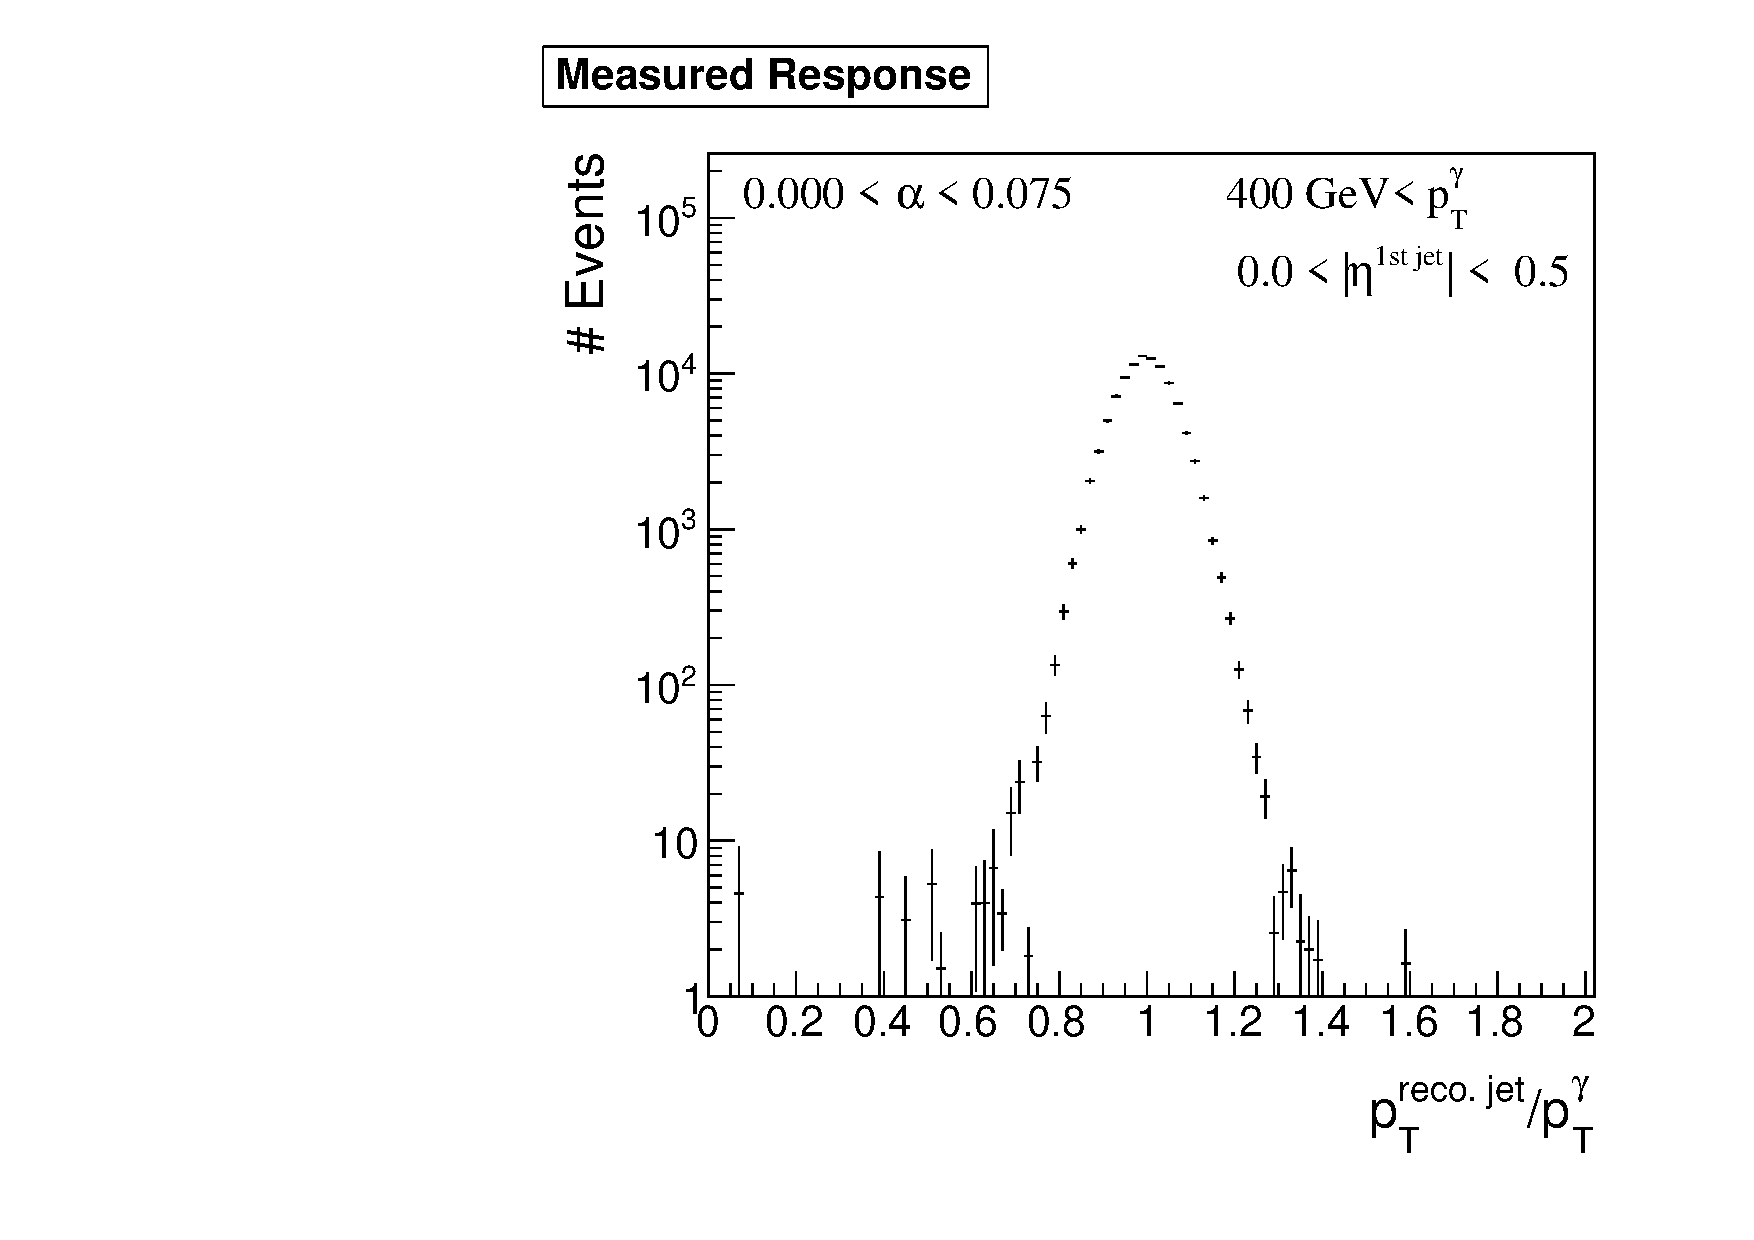
\includegraphics[width=0.33\textwidth]{figures/resolution/methodology/fullResponseExample1stBin.pdf}
     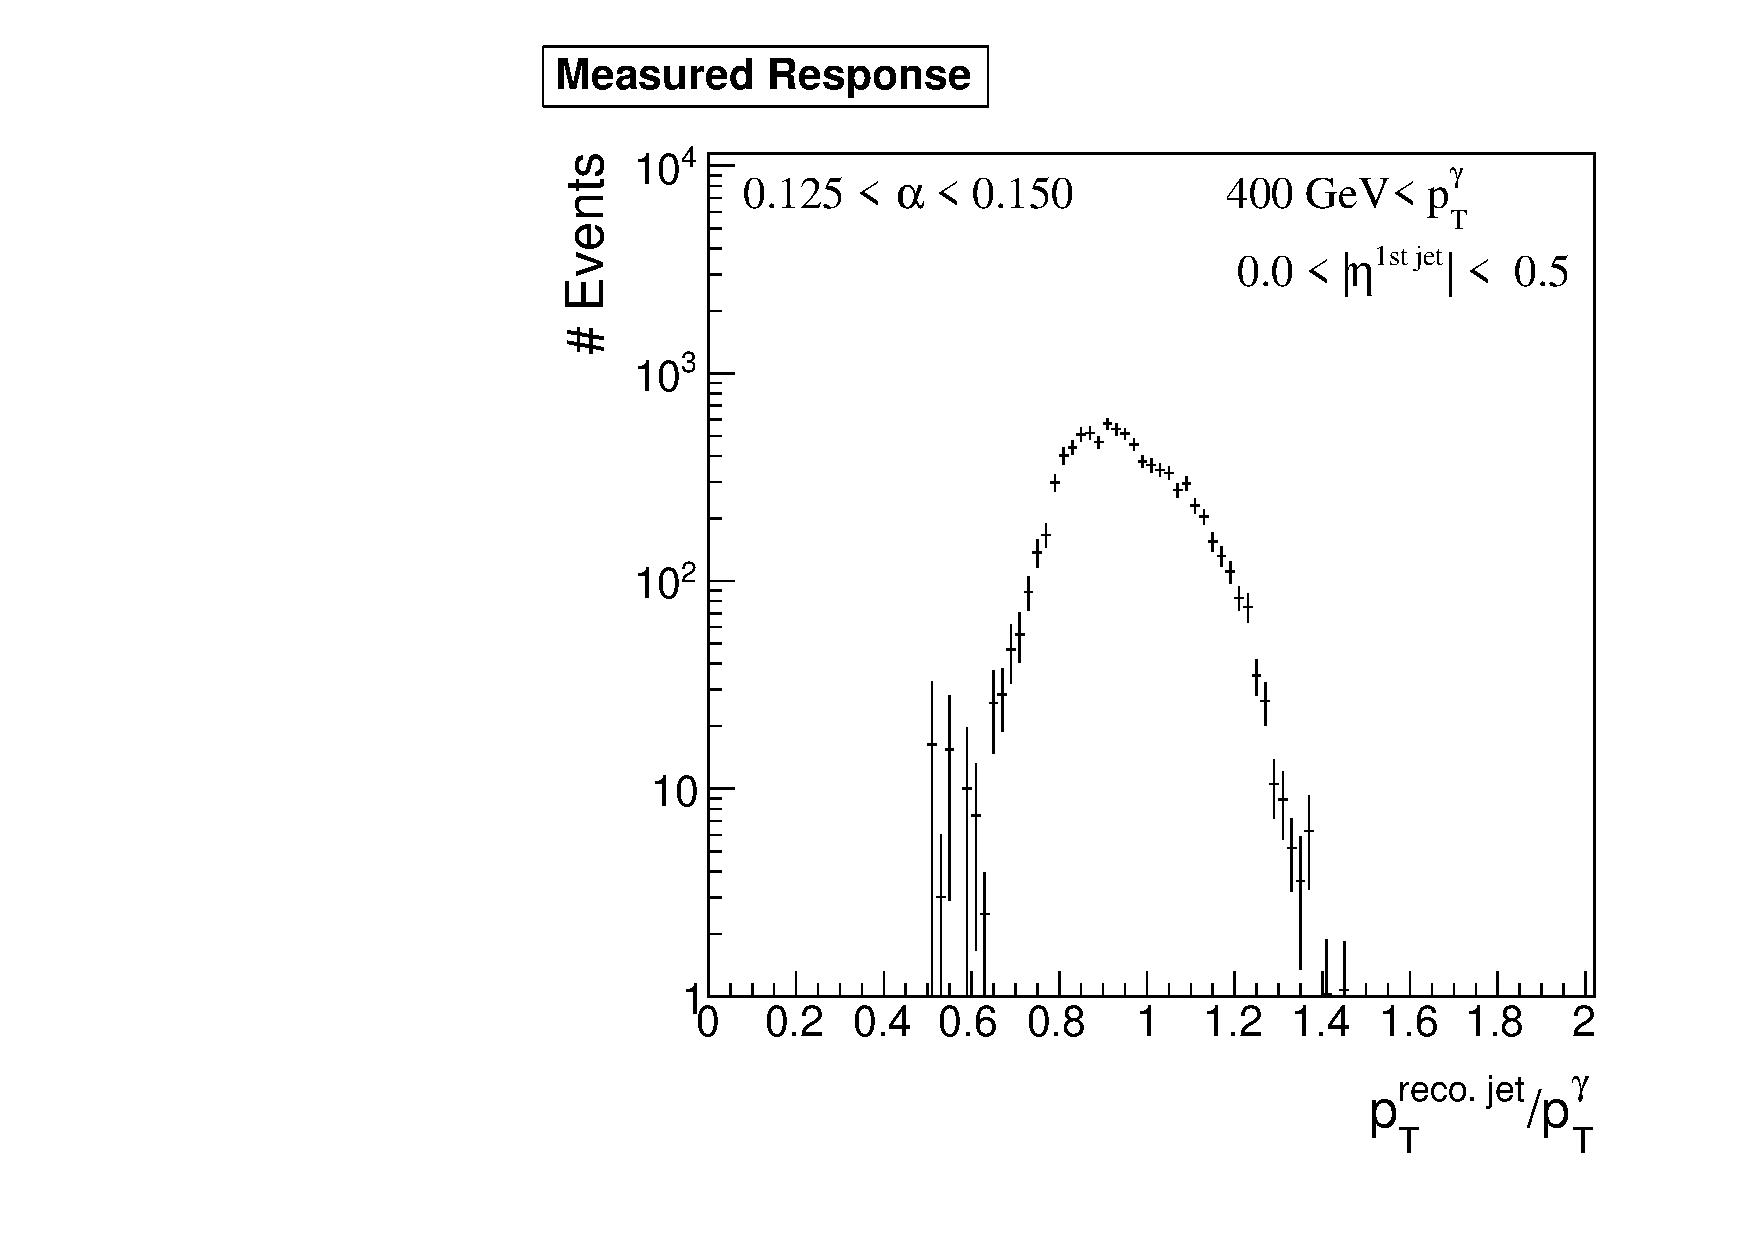
\includegraphics[width=0.33\textwidth]{figures/resolution/methodology/fullResponseExample4thBin.pdf}
     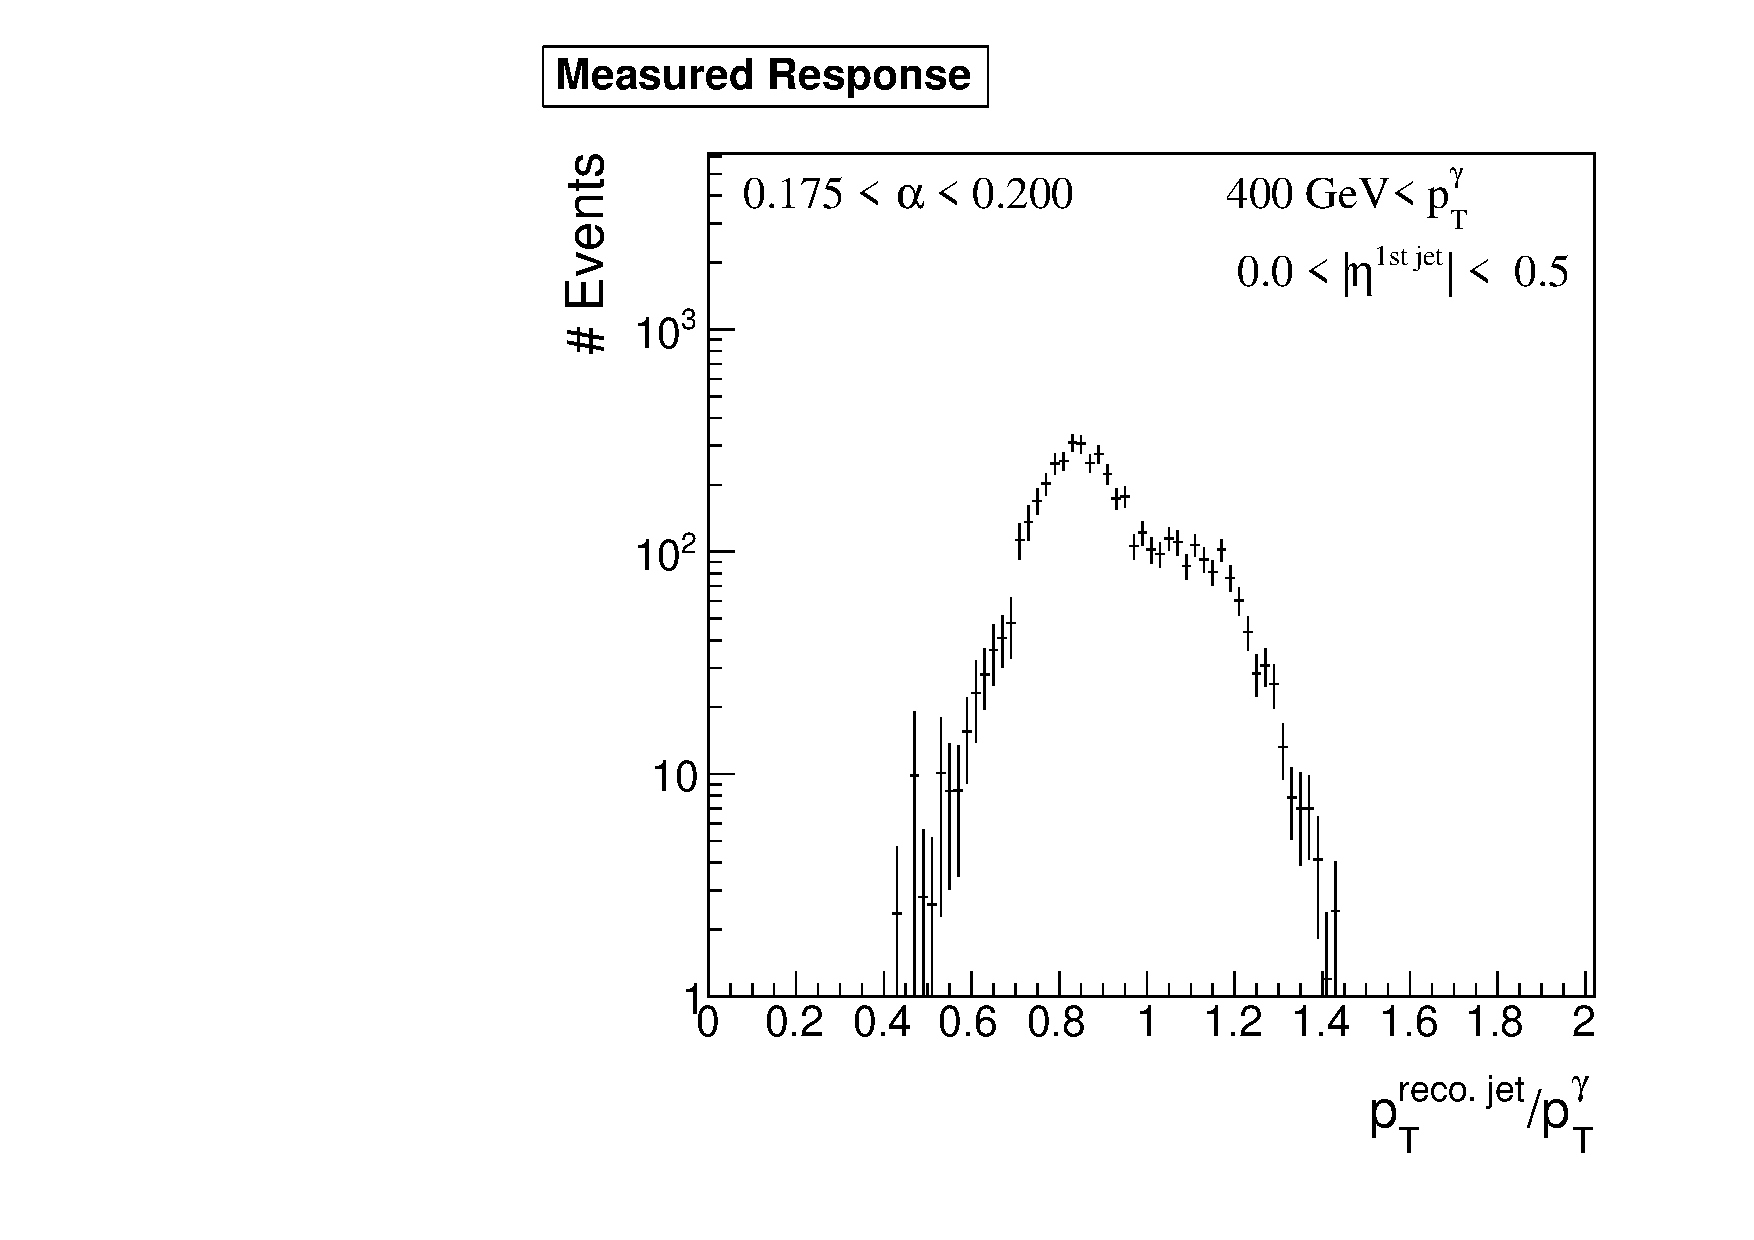
\includegraphics[width=0.33\textwidth]{figures/resolution/methodology/fullResponseExample6thBin.pdf}
  \caption{The measured response $\frac{\pt^{\text{reco. jet}}}{\pt^{\gamma}}$ in simulation for $\pt^{\gamma} < 400 \gev$ for three different $\alpha$ ranges: 
           (left) 0.0\%-7.5\%, (middle) 12.5\%-15.0\% and (right) 17.5\%-20.0 \%. 
           It can be seen that the double peak structure gets less pronounced for low $\alpha$ values.}  
 \label{fig:alphaBins}
\end{figure}

These two different contributions (second jet in photon/leading jet hemisphere) result in two separate response distribution.
A schematic sketch of the two contributions is shown in \mbox{Fig. \ref{fig:sketch}}. 

\begin{figure}[b]
 \centering
     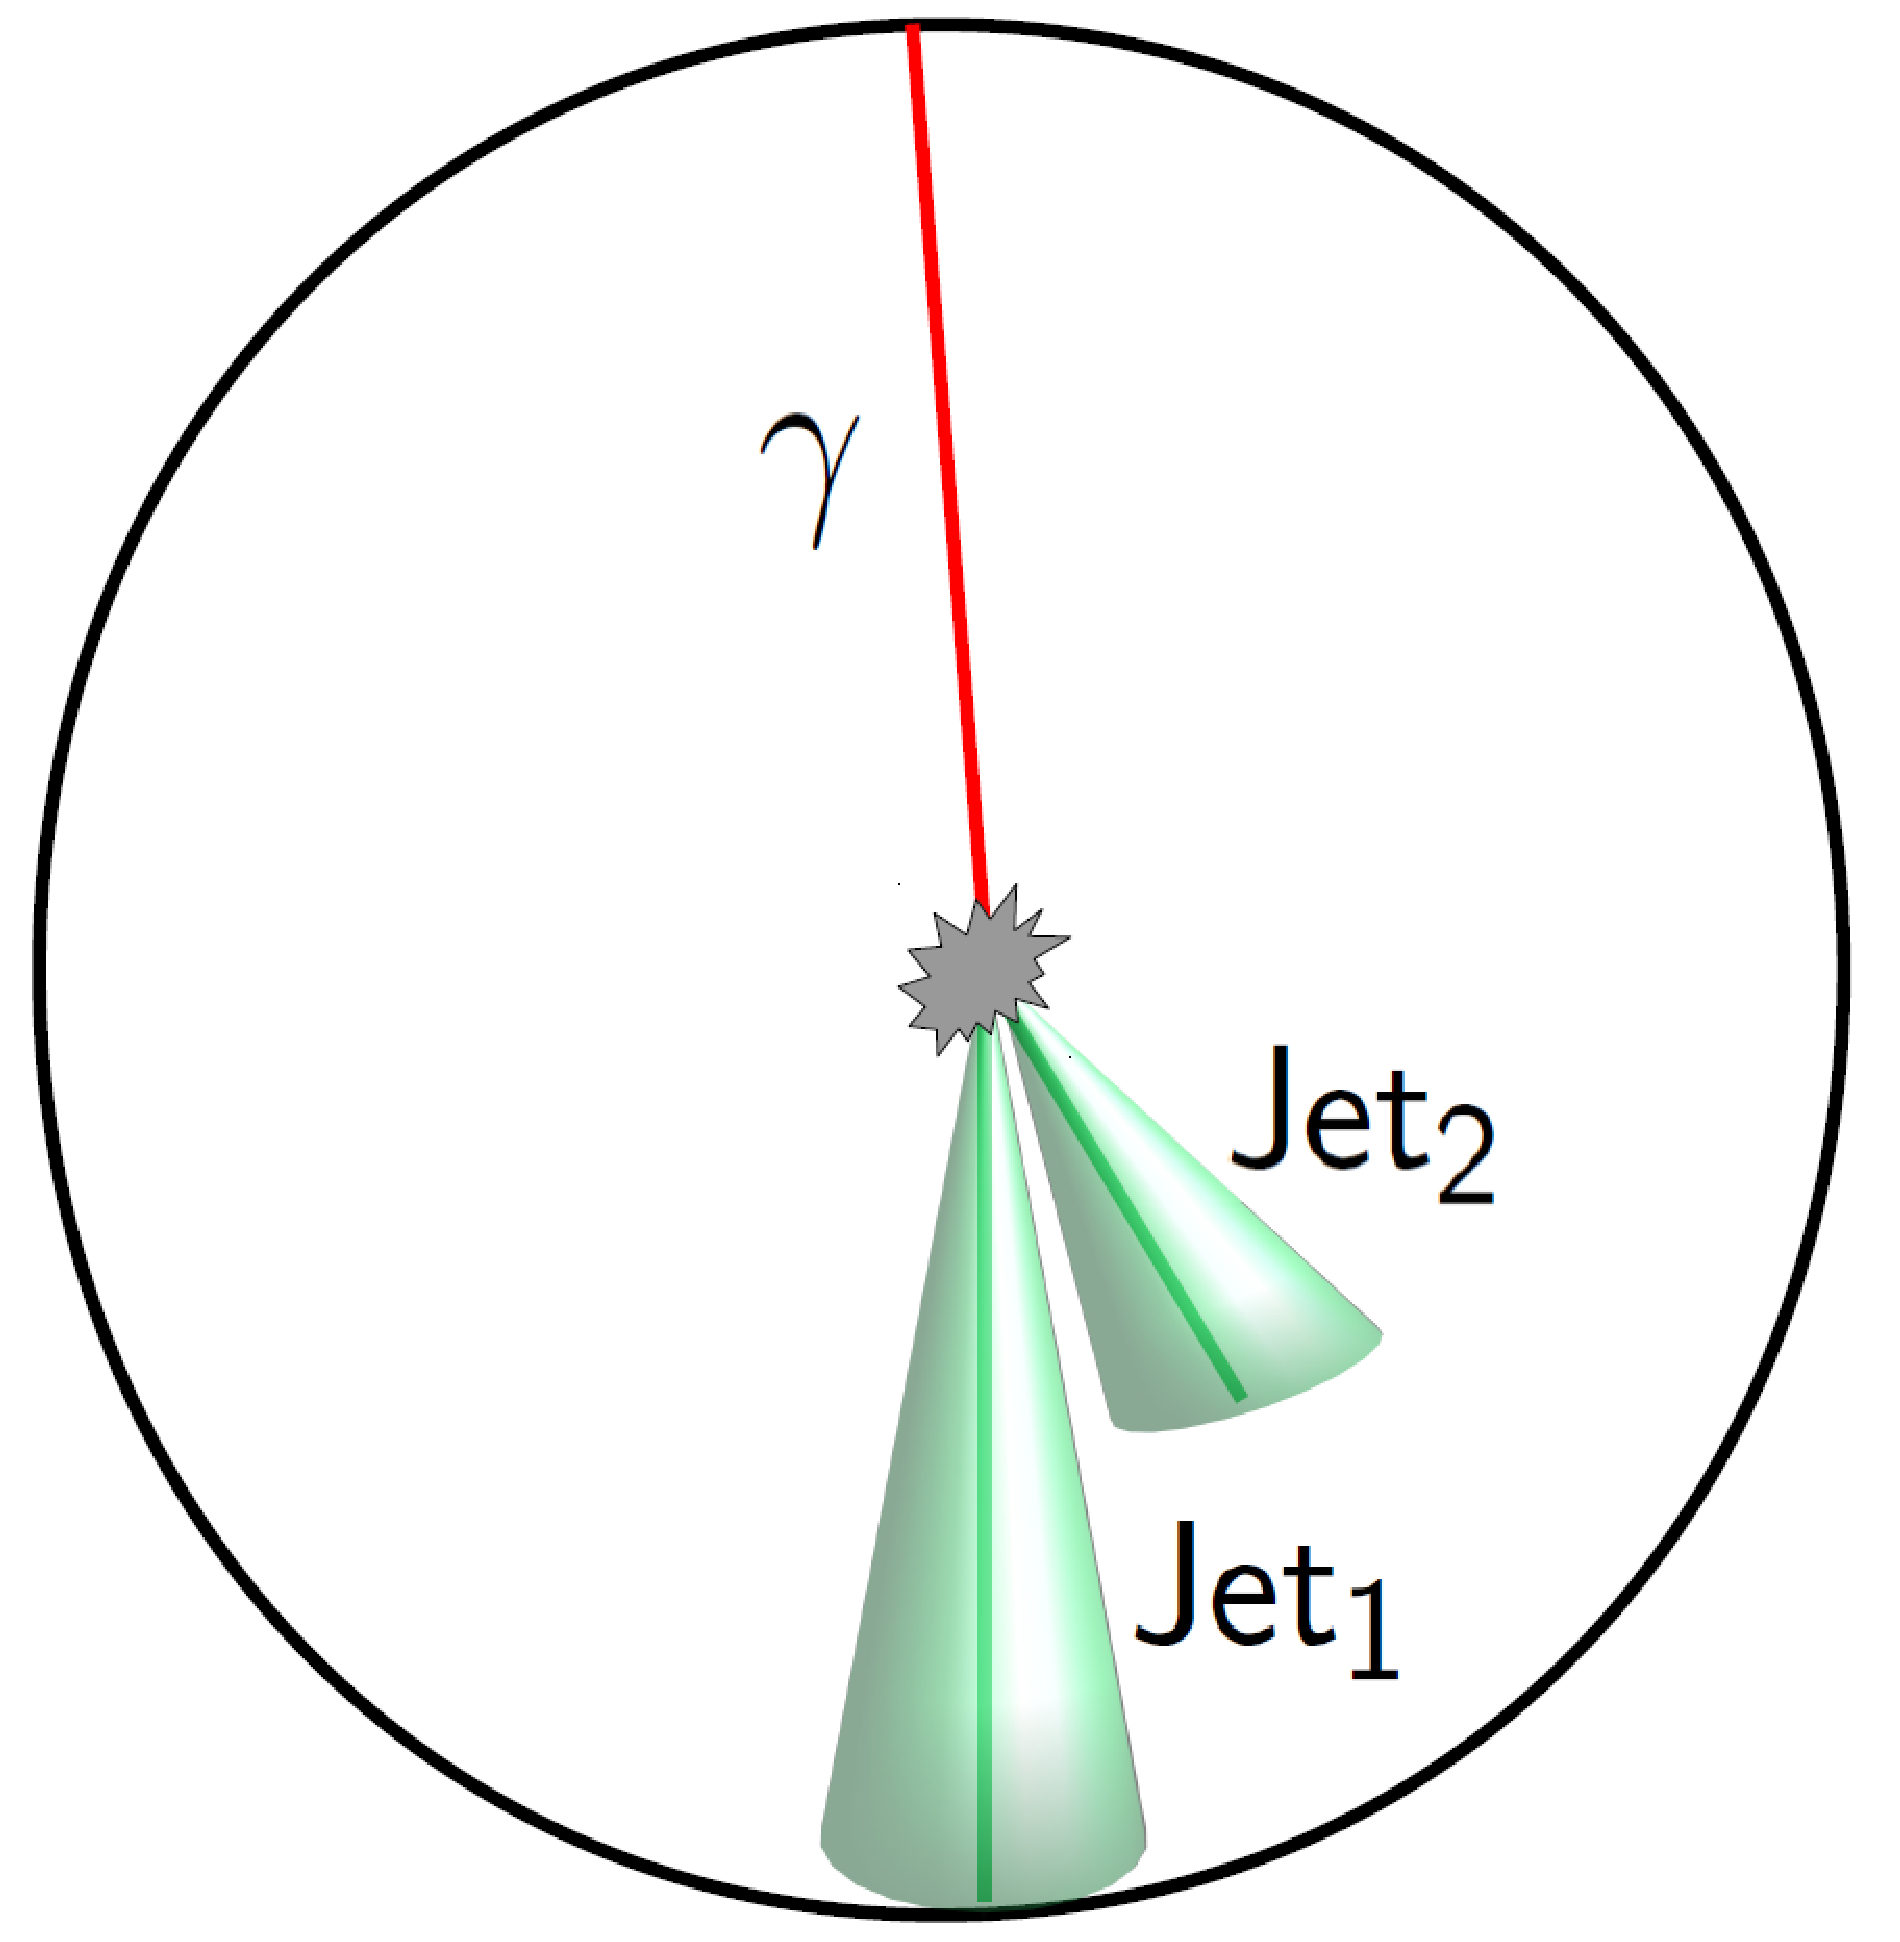
\includegraphics[width=0.49\textwidth]{figures/resolution/methodology/2ndJet_in_JetHemisphere.pdf}
     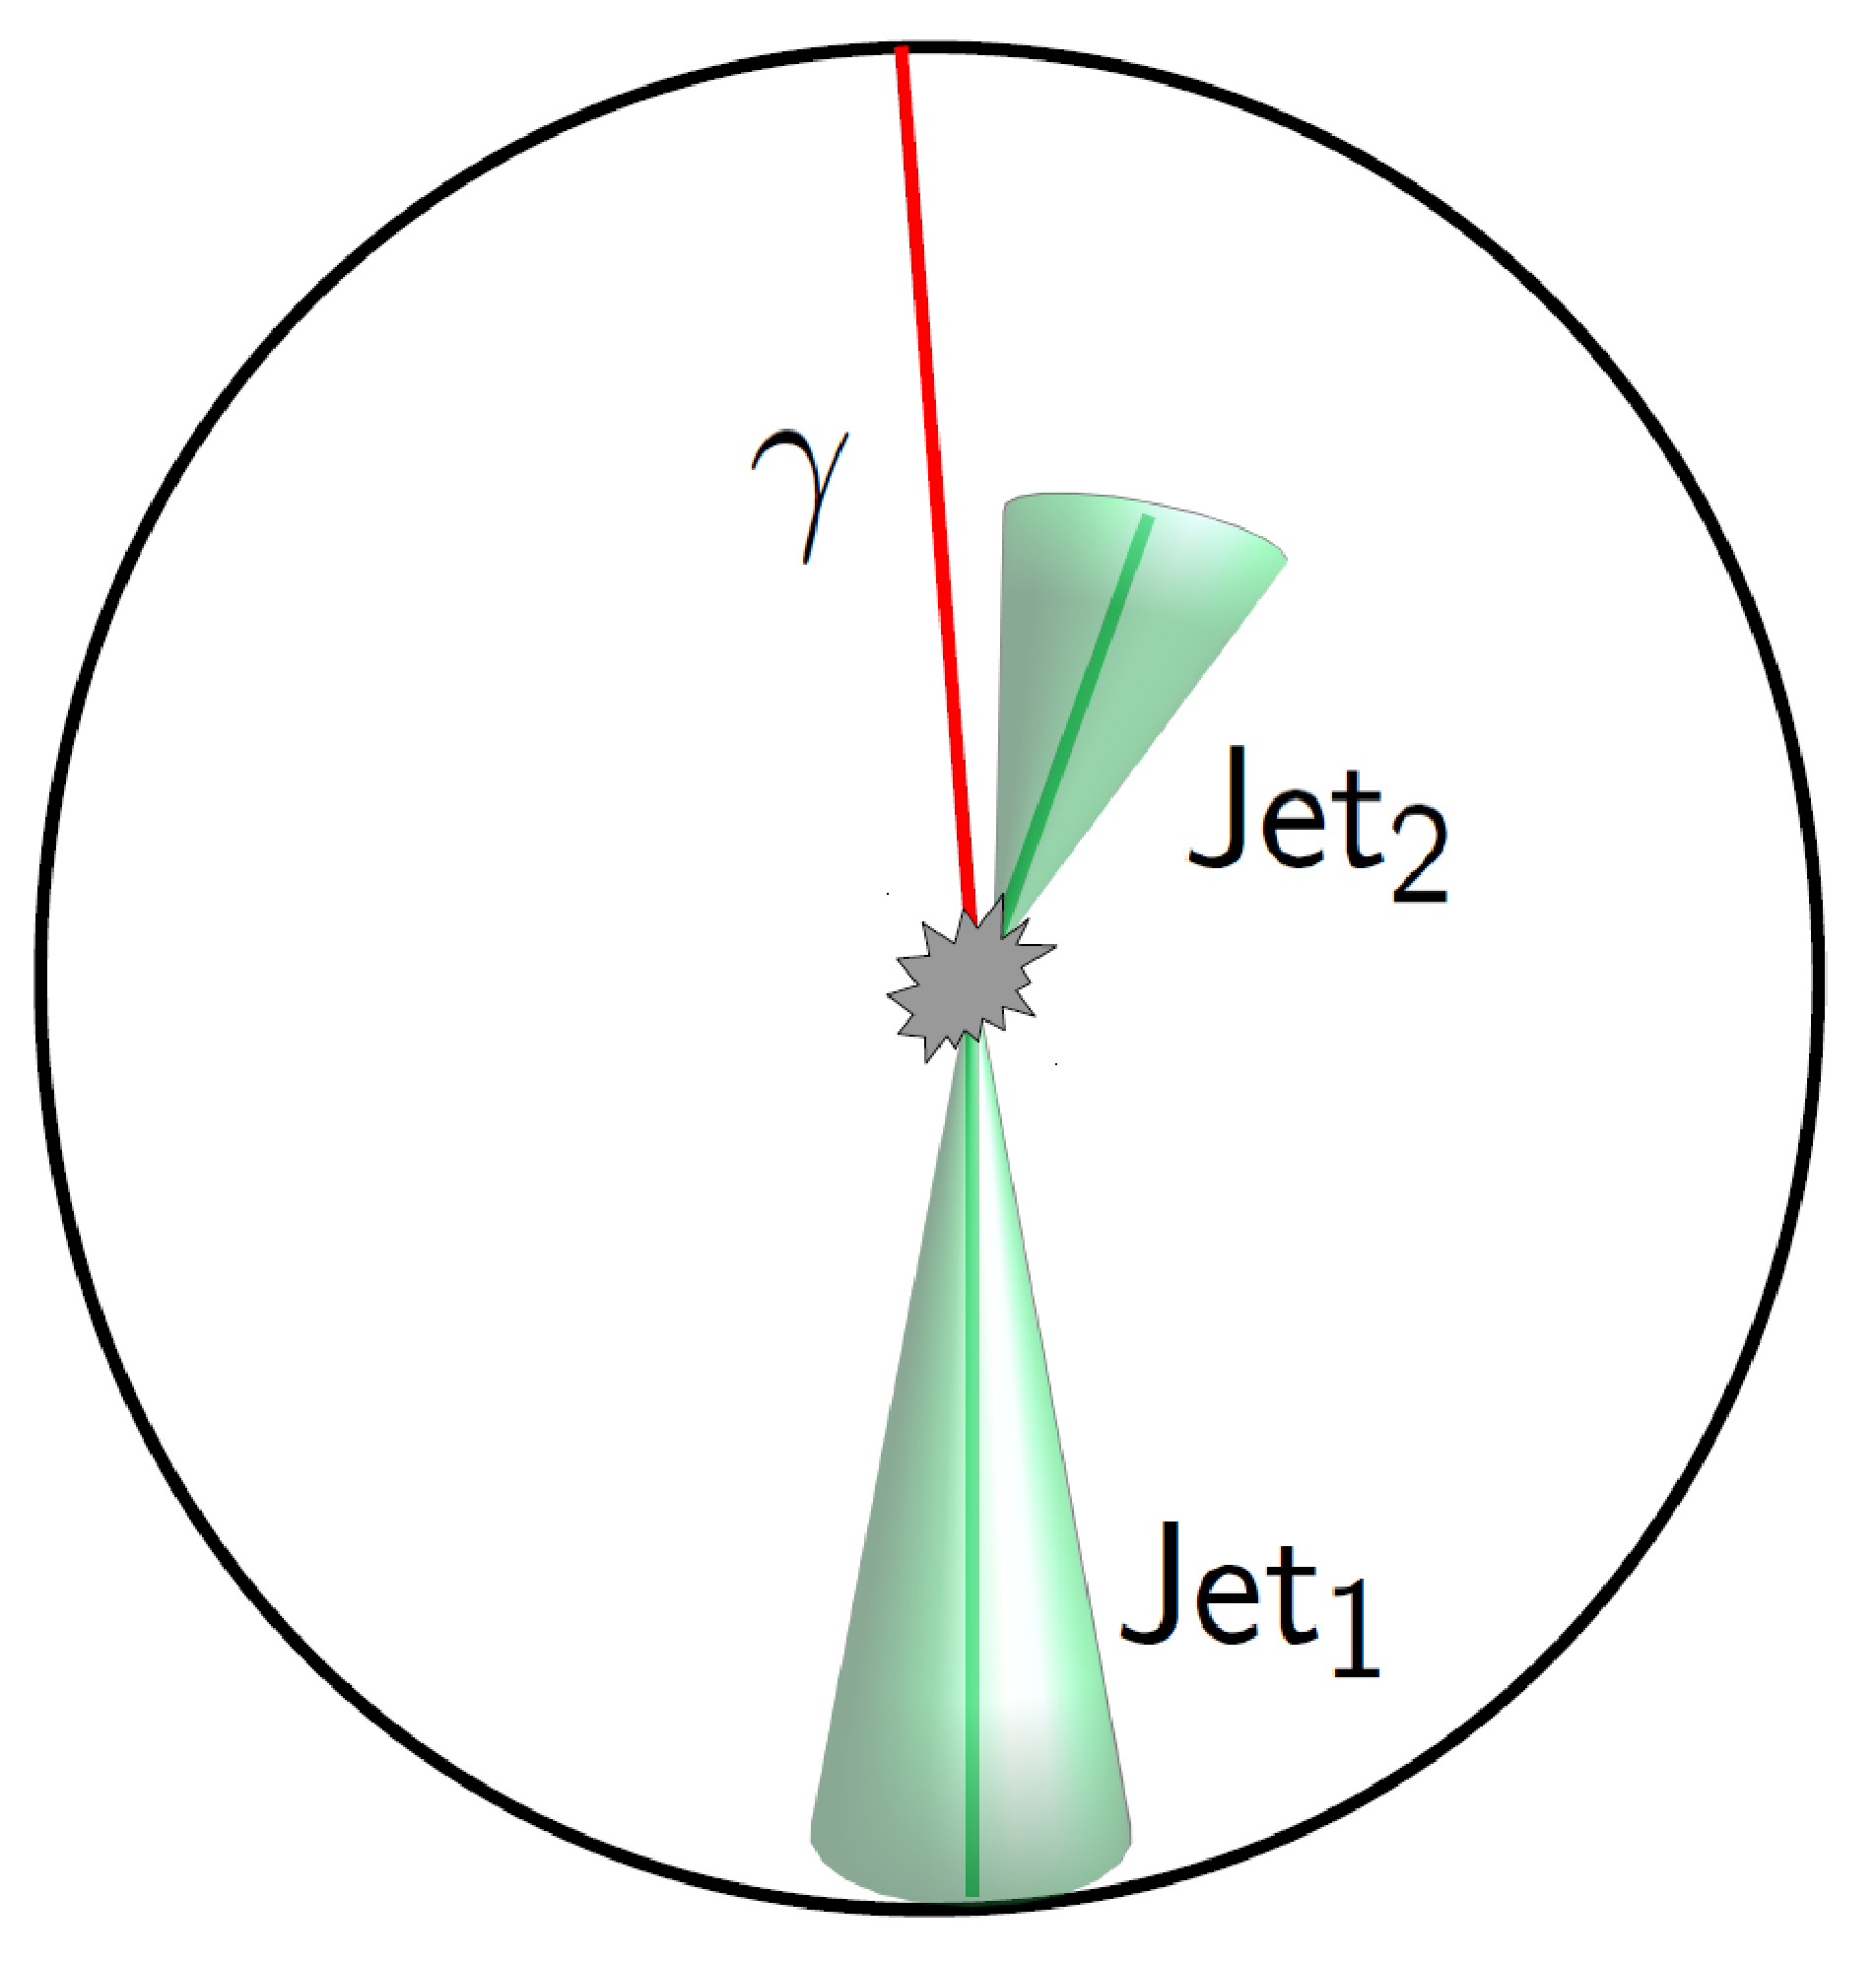
\includegraphics[width=0.49\textwidth]{figures/resolution/methodology/2ndJet_in_PhotonHemisphere.pdf}
  \caption{A schematic sketch of the two different event topologies where the second jet is in the leading jet (left) or the photon hemisphere (right)}  
 \label{fig:sketch}
\end{figure}

The mathematical definitions of the hemispheres are as follows:

\begin{equation}\label{eq:HemisphereDefinition}
\text{Hemisphere} = \begin{cases}
  \text{Jet},    & \Delta \Phi \left( \text{1st jet, 2nd jet} \right) < \Delta \Phi \left( \gamma \text{, 2nd jet} \right) , \\
  \text{Photon}, & \text{else}.\\
\end{cases}
\end{equation}

The two response distributions coming from the different event topologies are separately evaluated. First, the resolution is determined for each of the configurations 
(\mbox{cf. Fig. \ref{fig:fullResponseAndContributions}}), and then, the 
weighted mean of the two contributions is calculated.

As can be seen in \mbox{Fig. \ref{fig:fullResponseAndContributions}}, 
events containing a second jet in the leading jet hemisphere lead to a response histogram with mean smaller one, 
while events with a second jet in photon direction result in a distribution with mean larger one. 
The former occurs more frequently because it contains jets from final and initial state radiation, while
the latter mainly consists only from initial state radiation.

\begin{figure}[tbp]
  \centering

      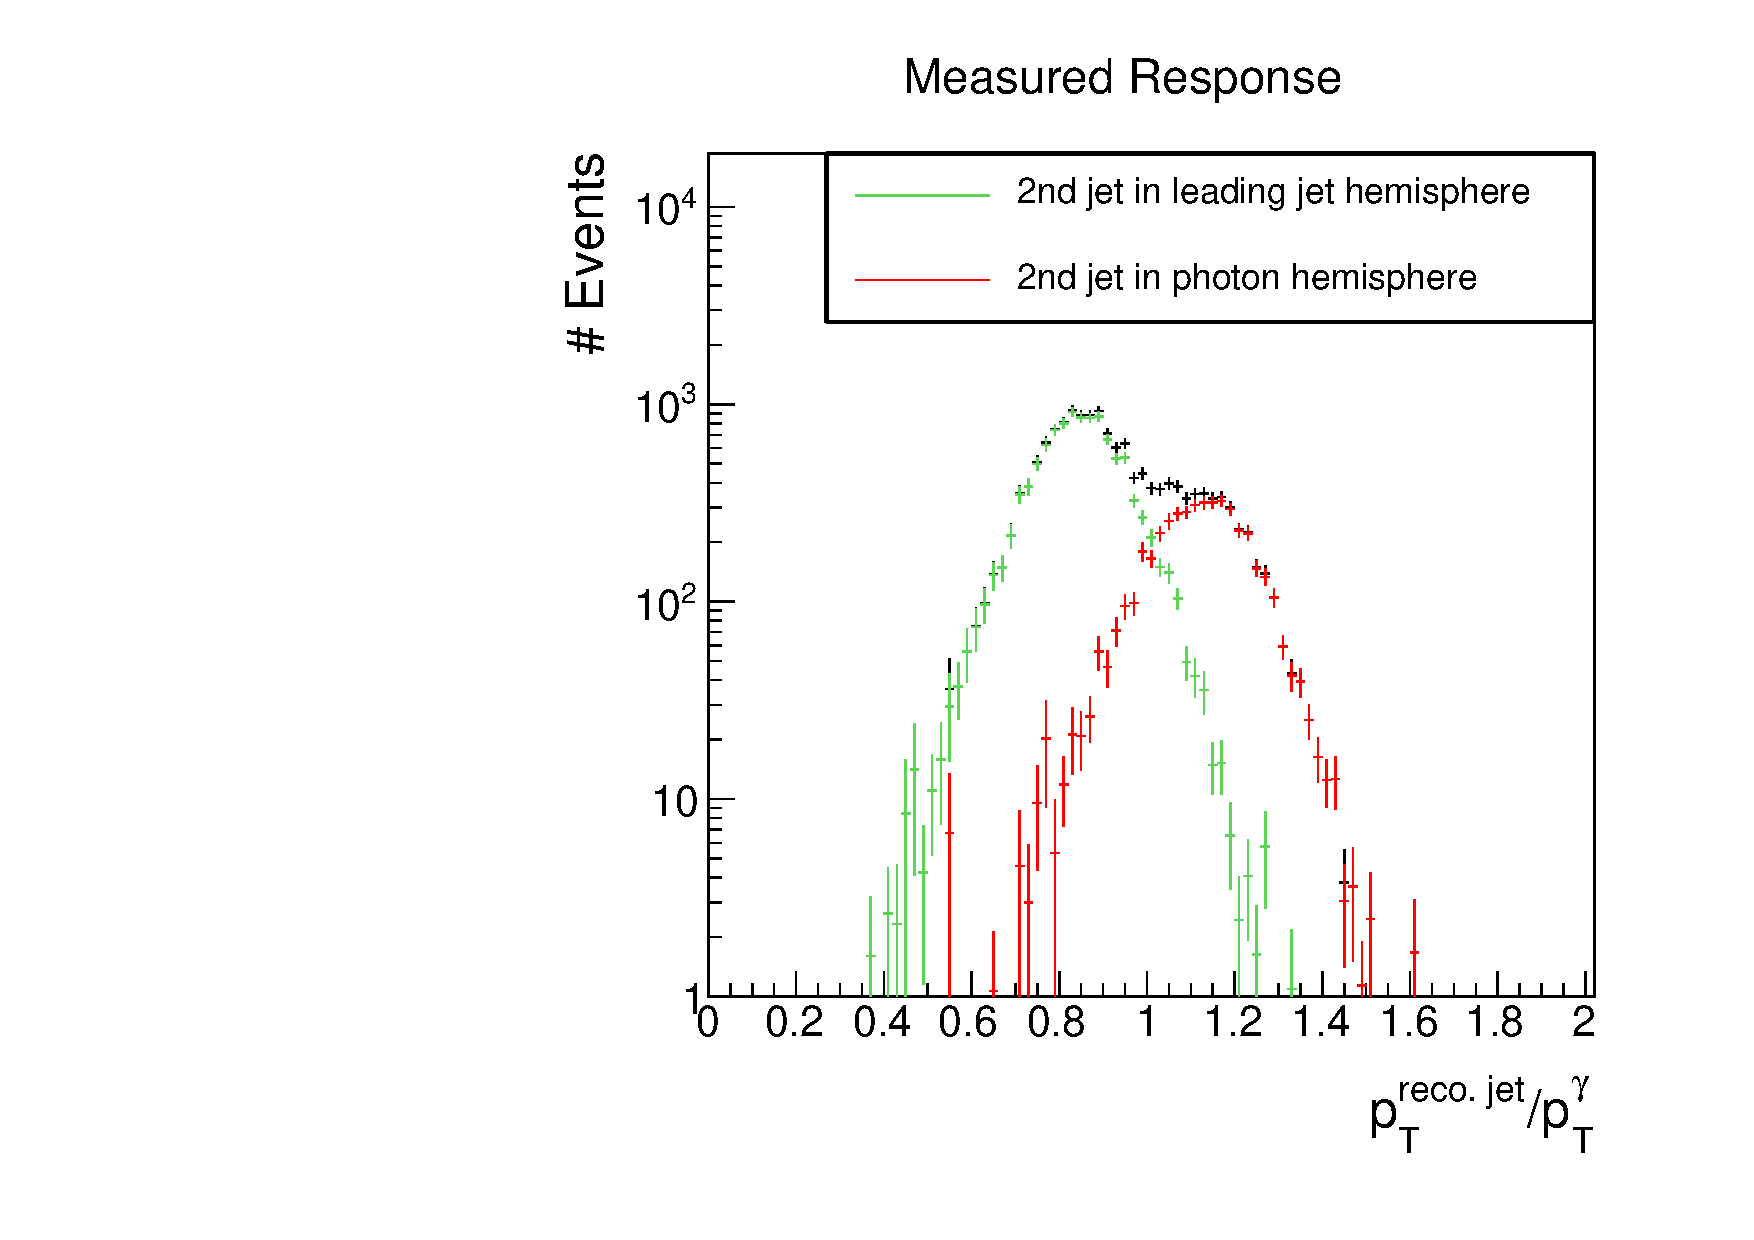
\includegraphics[width=0.49\textwidth]{figures/resolution/methodology/fullResponseAndContributionsExample.pdf}
 
  \caption{The measured response with the two contributions visualized. Events with a second jet in photon hemisphere (red) lead to a mean response larger one, while events with a
           second jet in the leading jet hemisphere (green) have a mean smaller one.}  
  \label{fig:fullResponseAndContributions}
\end{figure}

The intrinsic part of the resolution for a given photon $\pt$ bin is independent of secondary jet energy and thus can be considered as a constant in terms of $\alpha$

\begin{equation}\label{eq:intrinsic}
  \text{JER}_{\text{intrinsic}} \left( \alpha\right) = c^{\prime}.
\end{equation}

This is not true for the imbalance part. It was found empirically that the $\alpha$ dependence of the imbalance can be described by a linear function 

\begin{equation}\label{eq:imbalance}
  \text{JER}_{\text{imbalance}} \left( \alpha\right) = q^{\prime} + m^{\prime} \, \alpha
\end{equation}

Considering these two contributions as independent and folding them, $\text{JER}_{\text{intr.}} \oplus \text{JER}_{\text{imb.}}$, result in the following formula of the total resolution

\begin{equation}\label{eq:total}
  \text{JER}_{\text{total}} \left( \alpha \right) = \sqrt{ c^{\prime 2} + q^{\prime 2}  + 2 q^{\prime} m^{\prime} \cdot \alpha +m^{\prime 2} \cdot \alpha^2}. 
\end{equation}


In \mbox{Fig. \ref{fig:AlphaDependenceOfResolutions}}, the $\alpha$ dependence of the imbalance, the intrinsic resolution, and the total resolution is shown for two example 
$\pt^{\gamma}$ regions in simulated events. 
\begin{figure}[tbp]
 \centering
    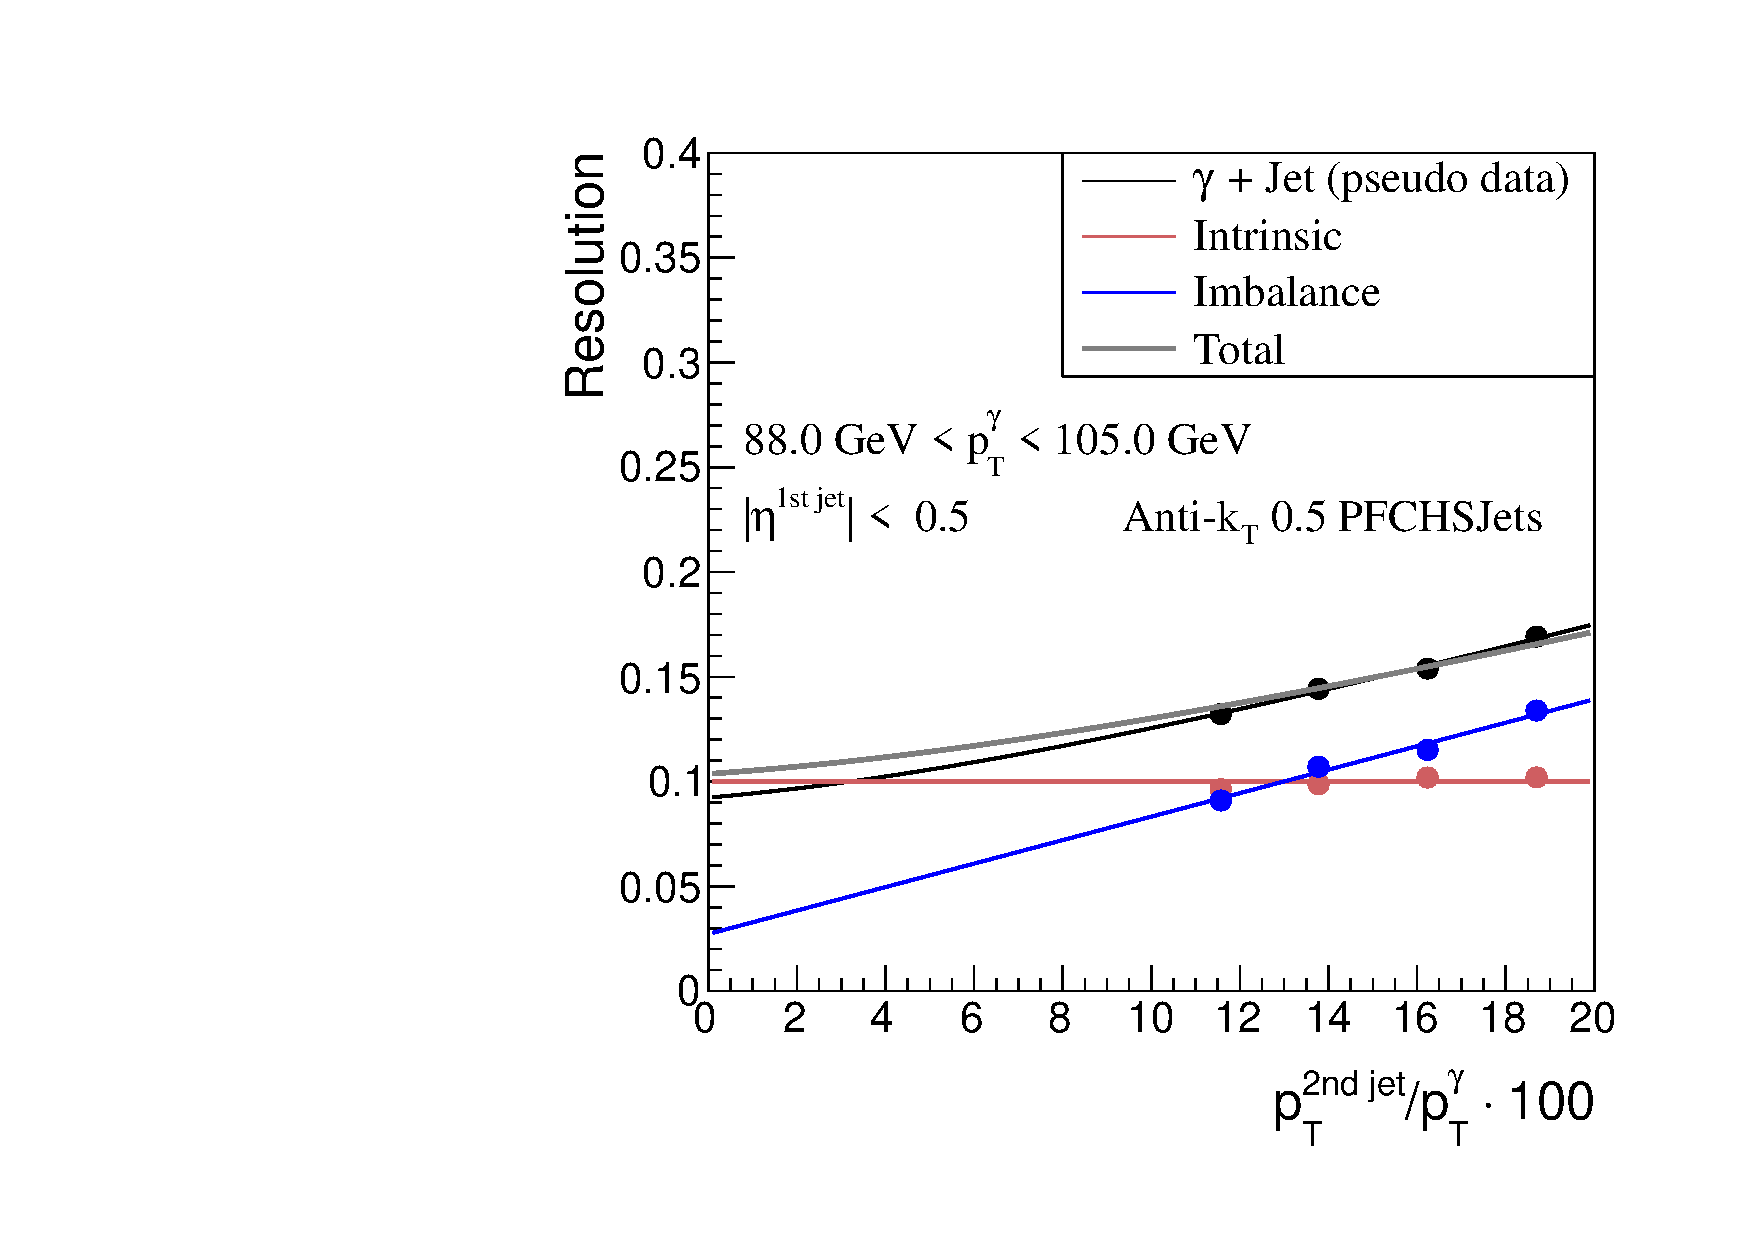
\includegraphics[width=0.49\textwidth]{figures/resolution/methodology/JER_for_1_eta_bin_4_pTGamma_bin_all_contributions_PFCHS_RMS99_mc.pdf} 
    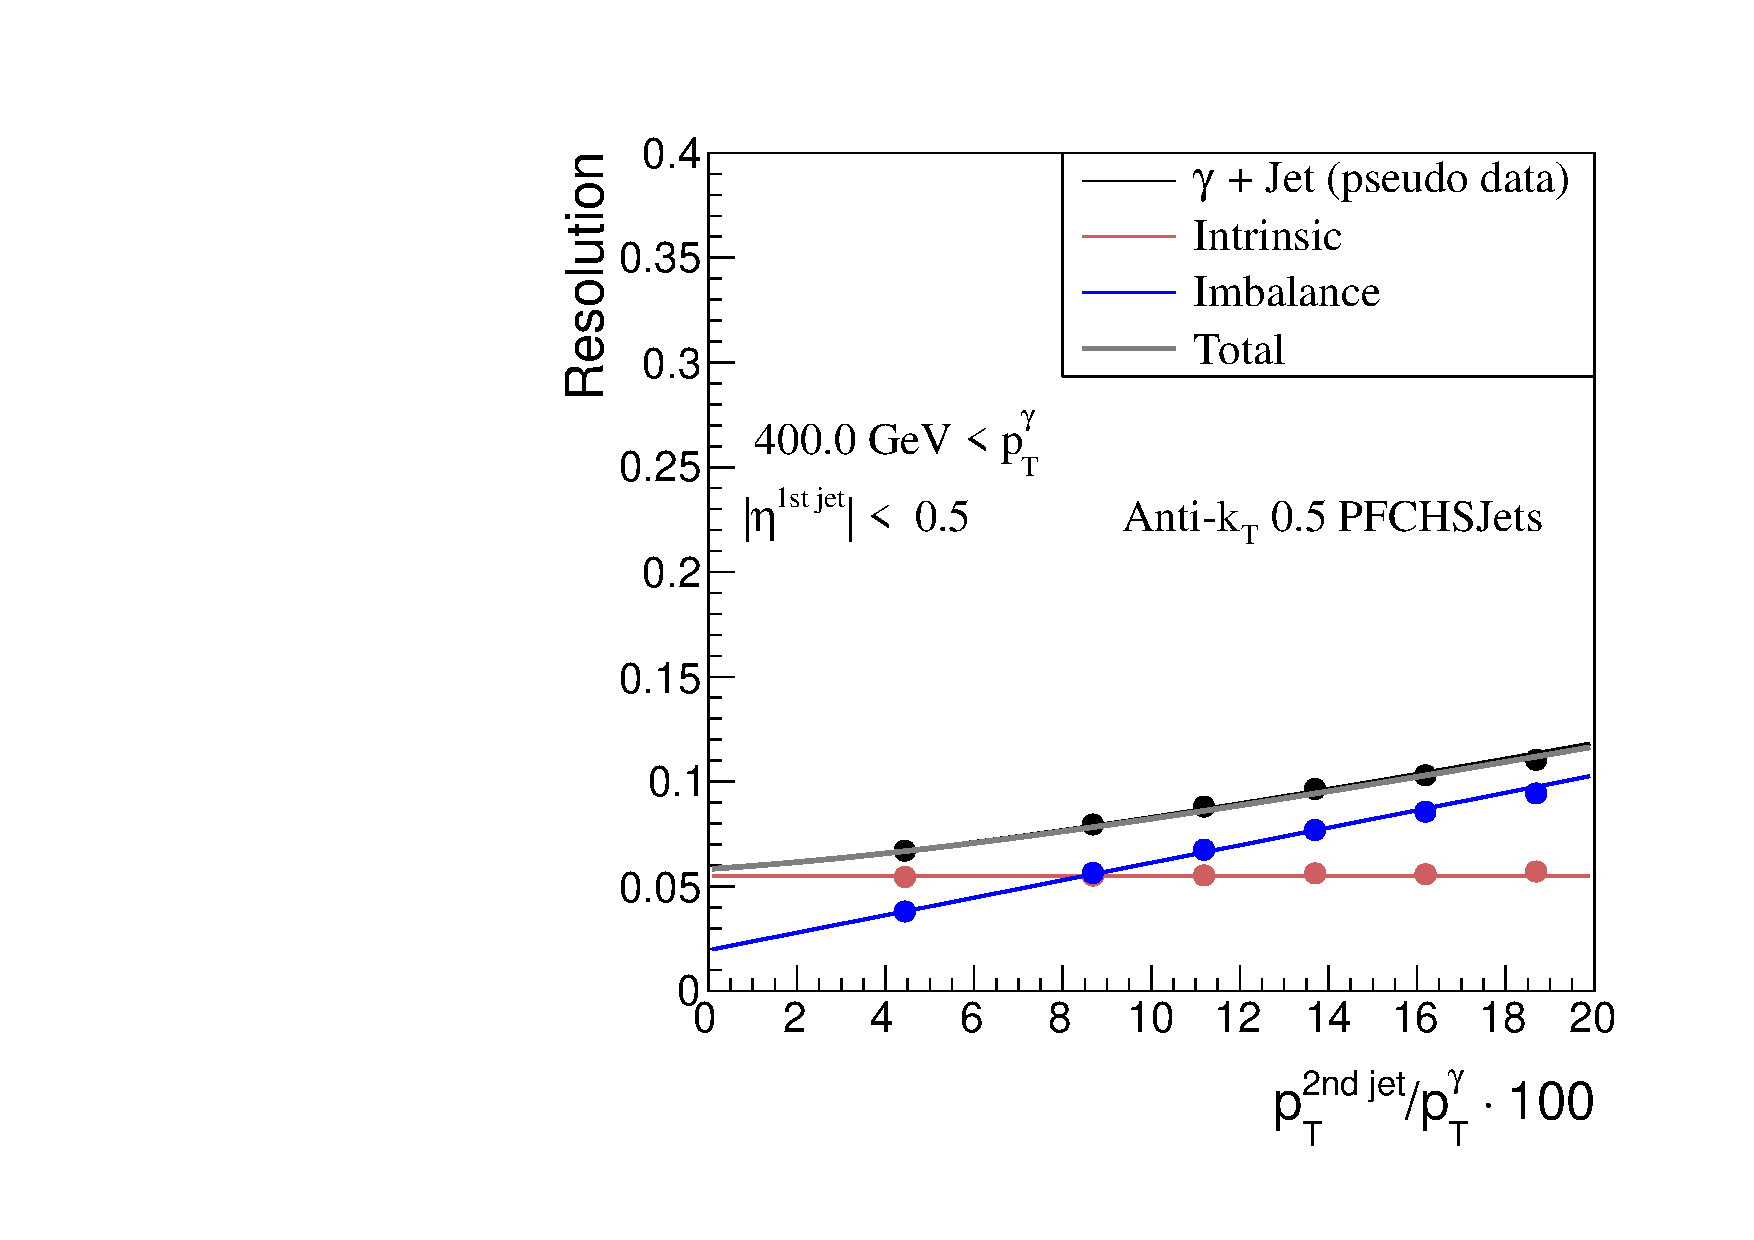
\includegraphics[width=0.49\textwidth]{figures/resolution/methodology/JER_for_1_eta_bin_12_pTGamma_bin_all_contributions_PFCHS_RMS99_mc.pdf} 
  \caption{The alpha dependency of the various parts of the resolution in the simulated events for (left) $83 \gev < \pt^{\gamma} < 99 \gev $ and (right) $400 \gev < \pt^{\gamma}$. The total resolution (Gray line) is the addition in quadrature of the imbalance (blue line) and the intrinsic (red line) 
  fit functions. It can 
  be compared to the measured pseudo data (black line).}  
 \label{fig:AlphaDependenceOfResolutions}
\end{figure}
The measured intrinsic resolution and imbalance for various $\alpha$ values are fitted with functions \eqref{eq:intrinsic} and \eqref{eq:imbalance}, respectively.
The measured total resolution (black dots) is fitted with function \eqref{eq:total}. Here, only $c^{\prime}$ and $m^{\prime}$ are free parameters, 
whereas $q^{\prime}$ is fixed to the value obtained from the imbalance fit. 
All contributions are well described by their fit functions. 
The gray line is the total resolution with the analytic expression of function \eqref{eq:total} with the parameters set to the fit values of the intrinsic and the imbalance fit. 

It is apparent that the imbalance is not zero for $\alpha=0$. This has two reasons.
First and most important, only the photon and the parton are balanced in the transverse plane, 
not necessarily the particles which are measured in the detector after hadronization. 
Because of the necessity of a jet reconstruction algorithm (Anti-k$_{\text{t}}$ in this analysis) with finite cone size, 
it can happen that not all particles which belong to a jet are covered by 
that algorithm (out-of-cone showering) and the photon and the particle-level jet are not balanced anymore (even for $\alpha = 0$). Second, also the photon \pt can 
be wrongly measured and spoil the residual imbalance $q^{\prime}$. 

These two effects lead to a small discrepancy between the measured resolution (black) and the intrinsic (red) also for zero second jet energy. 
To correct for this effect,  $q^{\prime}$ is fixed to the value obtained 
from fitting the imbalance part of the resolution (Eq.~\eqref{eq:imbalance}) and then only the fit parameter  $c^{\prime}$ is taken as the relevant resolution from the fit.
Also for measured data, $q^{\prime}$ is fixed to the value obtained from simulation. 
\mbox{Figure \ref{fig:ImbalanceOfPtgamma}} shows the residual imbalance for two exemplary $\eta^{\text{1st jet}}$ bins. 
It is almost stable and around 2\% over the whole photon \pt range.
\begin{figure}[tbp]
  \centering
    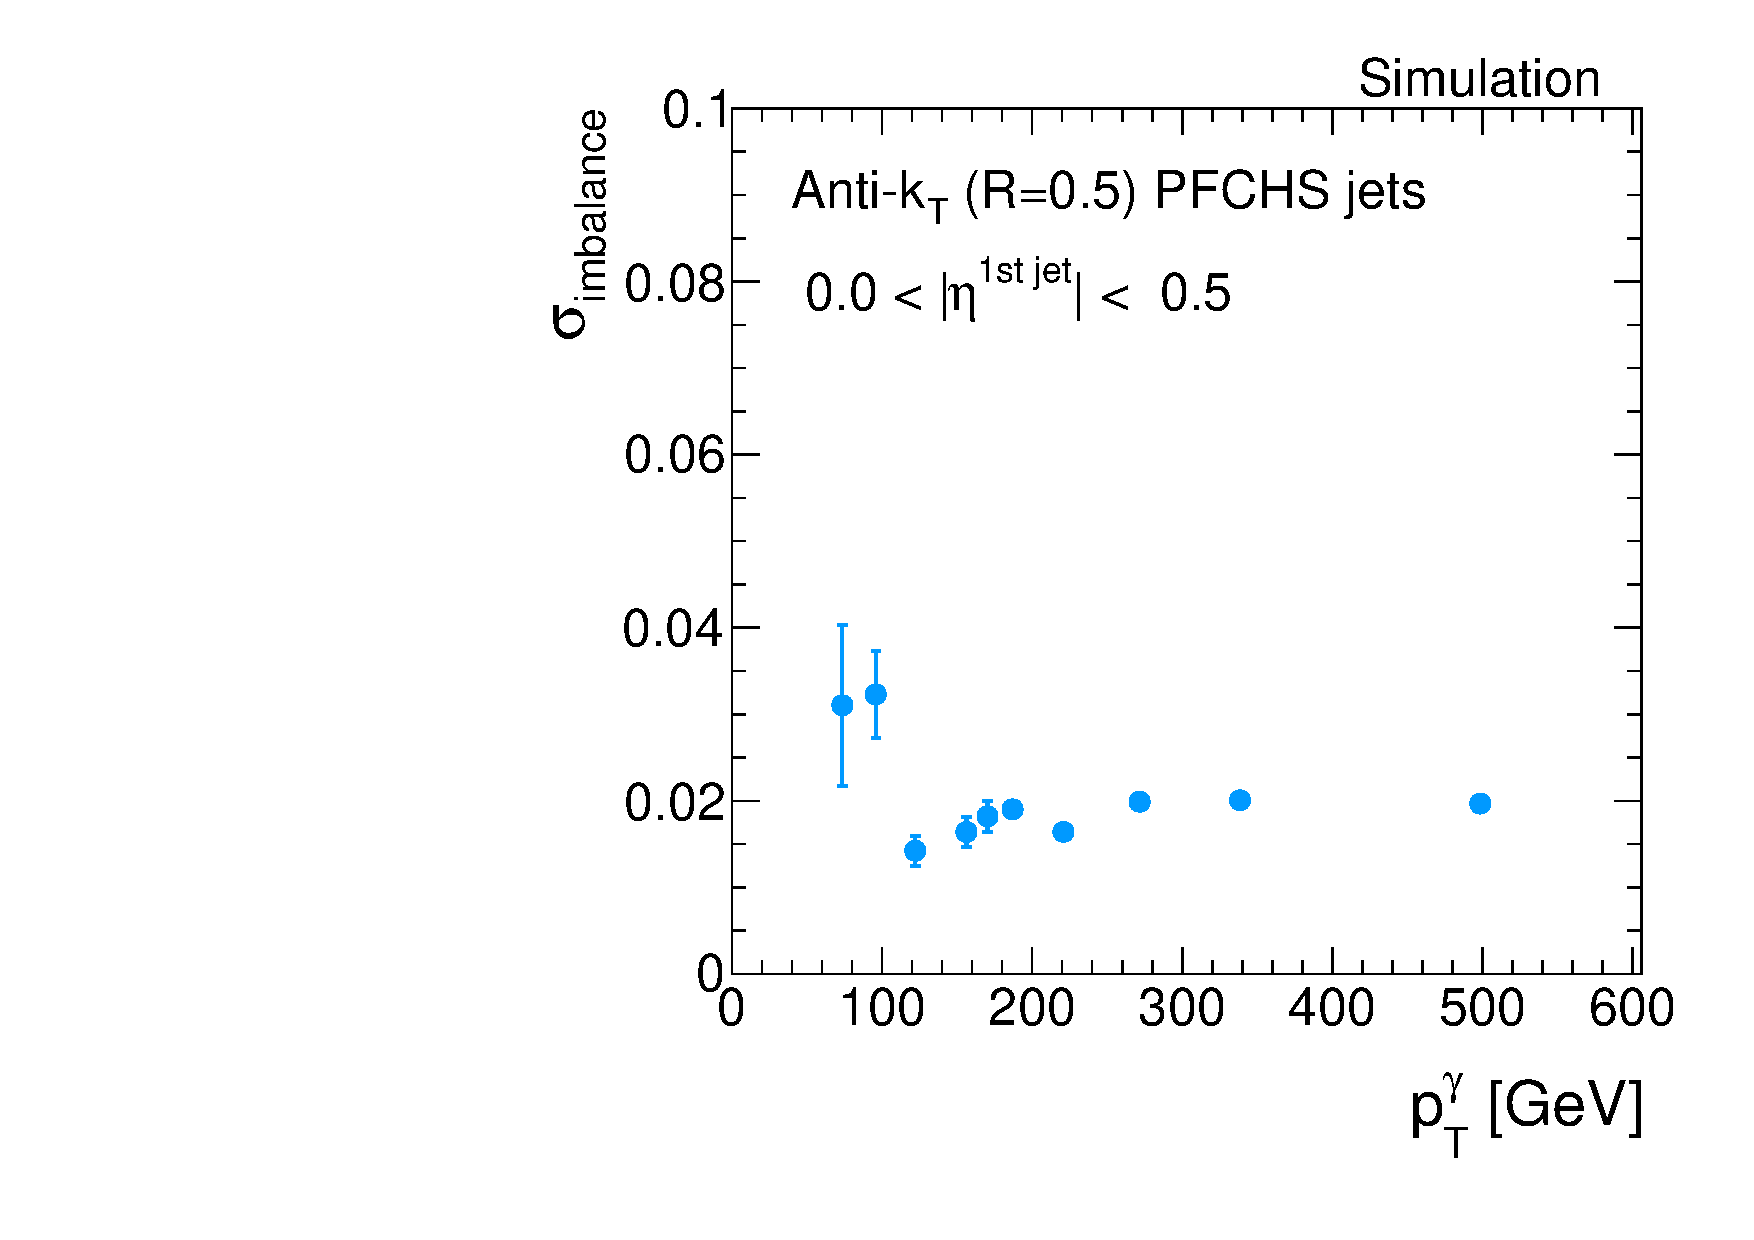
\includegraphics[width=0.49\textwidth]{figures/resolution/methodology/Imbalance_for_1_eta_bin_PFCHS_mc_RMS99.pdf}
    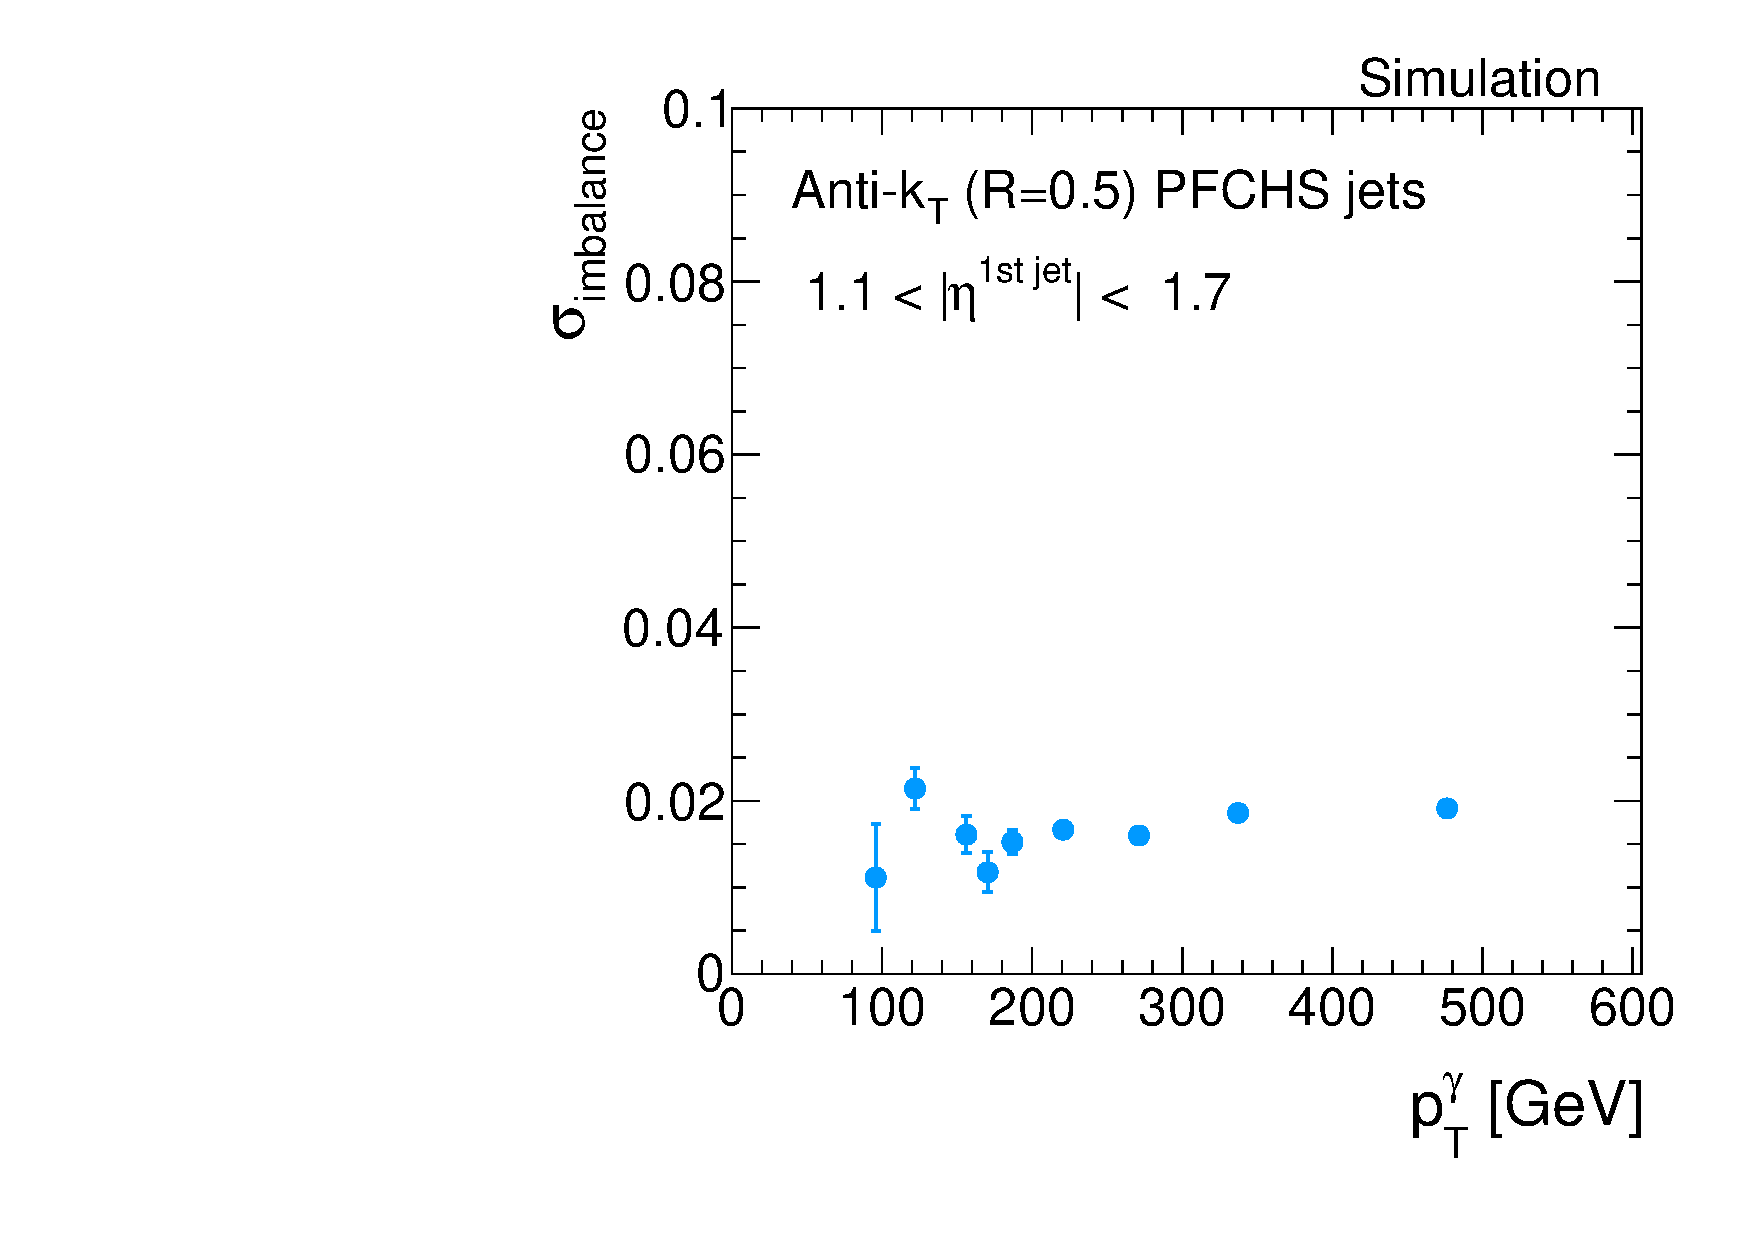
\includegraphics[width=0.49\textwidth]{figures/resolution/methodology/Imbalance_for_3_eta_bin_PFCHS_mc_RMS99.pdf}
  \caption{Imbalance for $|\eta^{\text{1st jet}}| < 0.5$ (left) and $1.1<|\eta^{\text{1st jet}}| < 1.7$ (right) in simulation.}  
  \label{fig:ImbalanceOfPtgamma}
\end{figure}

In \mbox{Fig. \ref{fig:ResolutionOfPtgamma}}, the fitted intrinsic resolution in simulation is shown in the different photon \pt bins for two different $\eta^{\text{1st jet}}$ regions.
The resolution improves for increasing photon \pt. 
\begin{figure}[tbp]
  \centering
    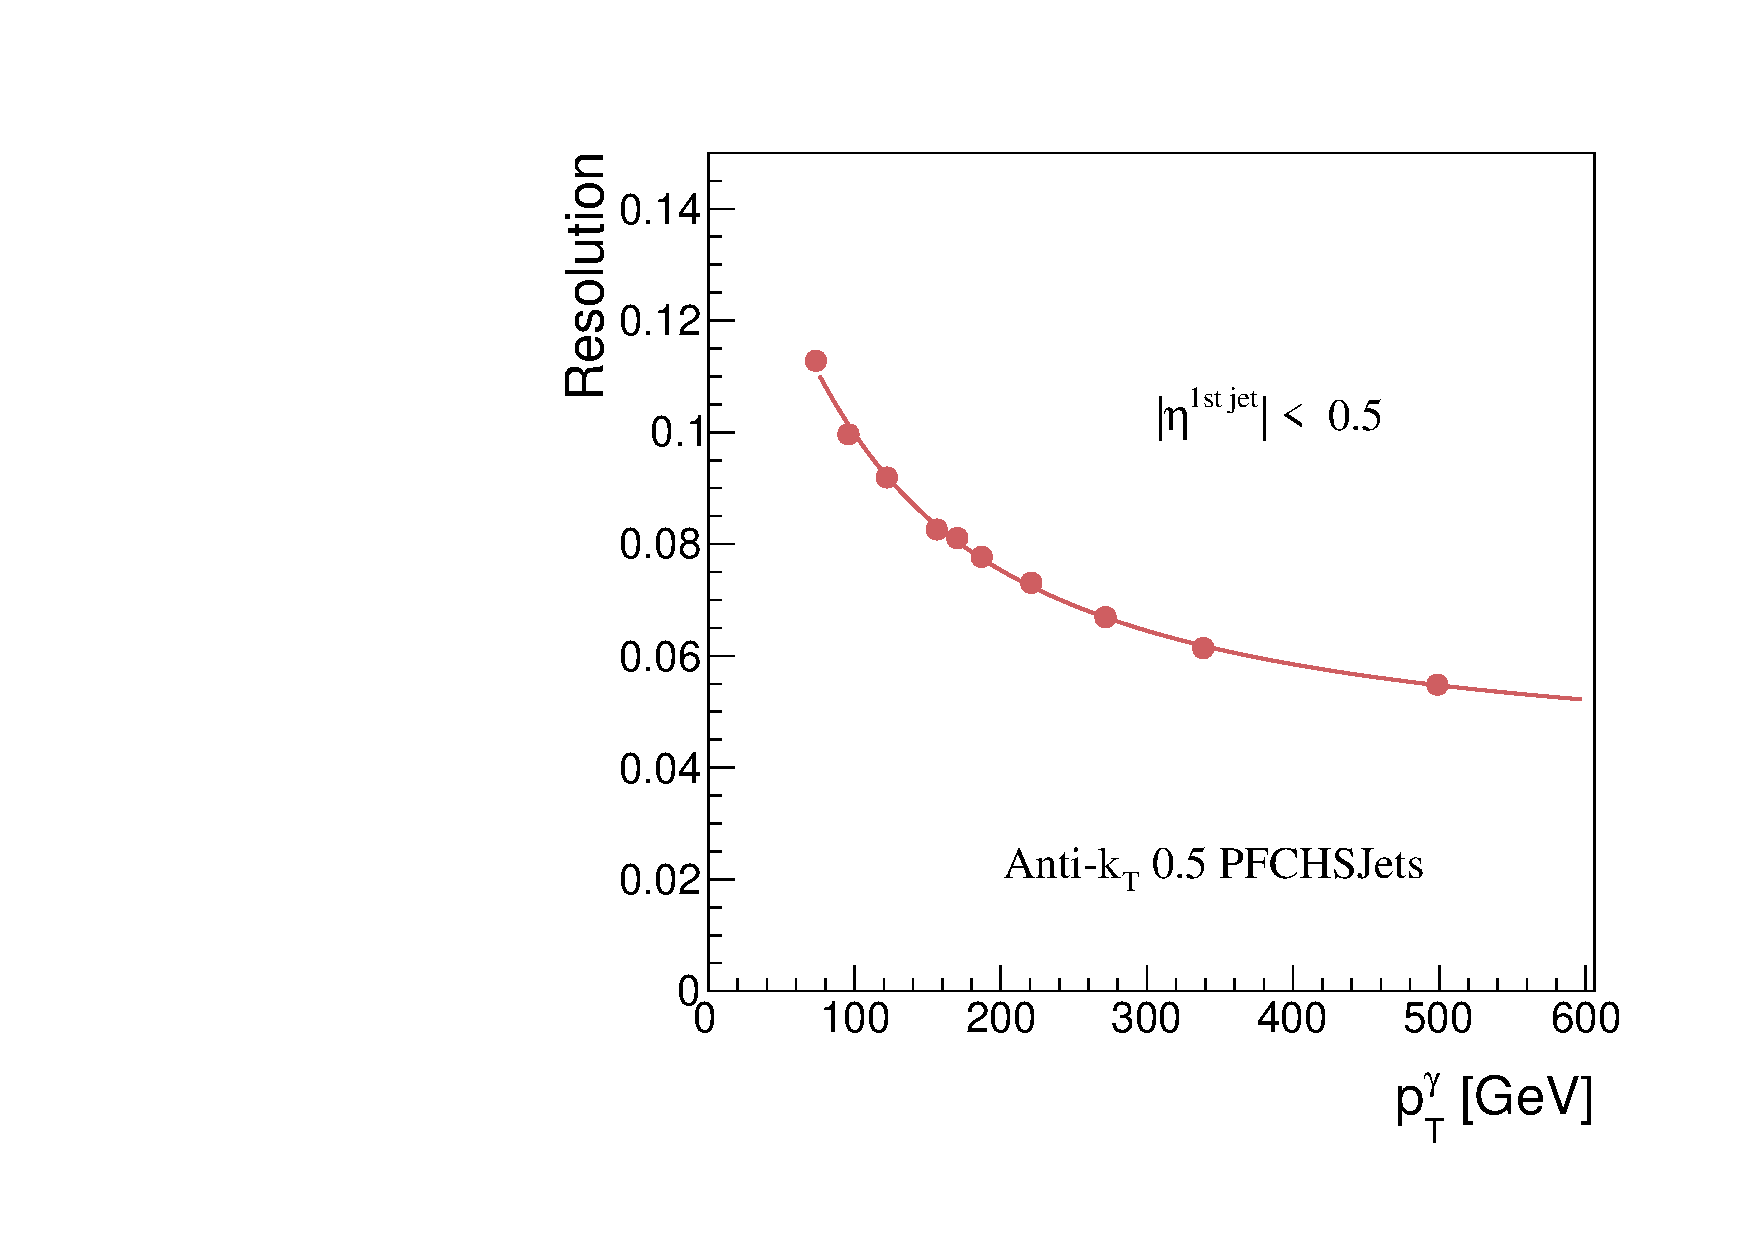
\includegraphics[width=0.49\textwidth]{figures/resolution/methodology/Resolution_for_1_eta_bin_PFCHS_mc_RMS99.pdf}
    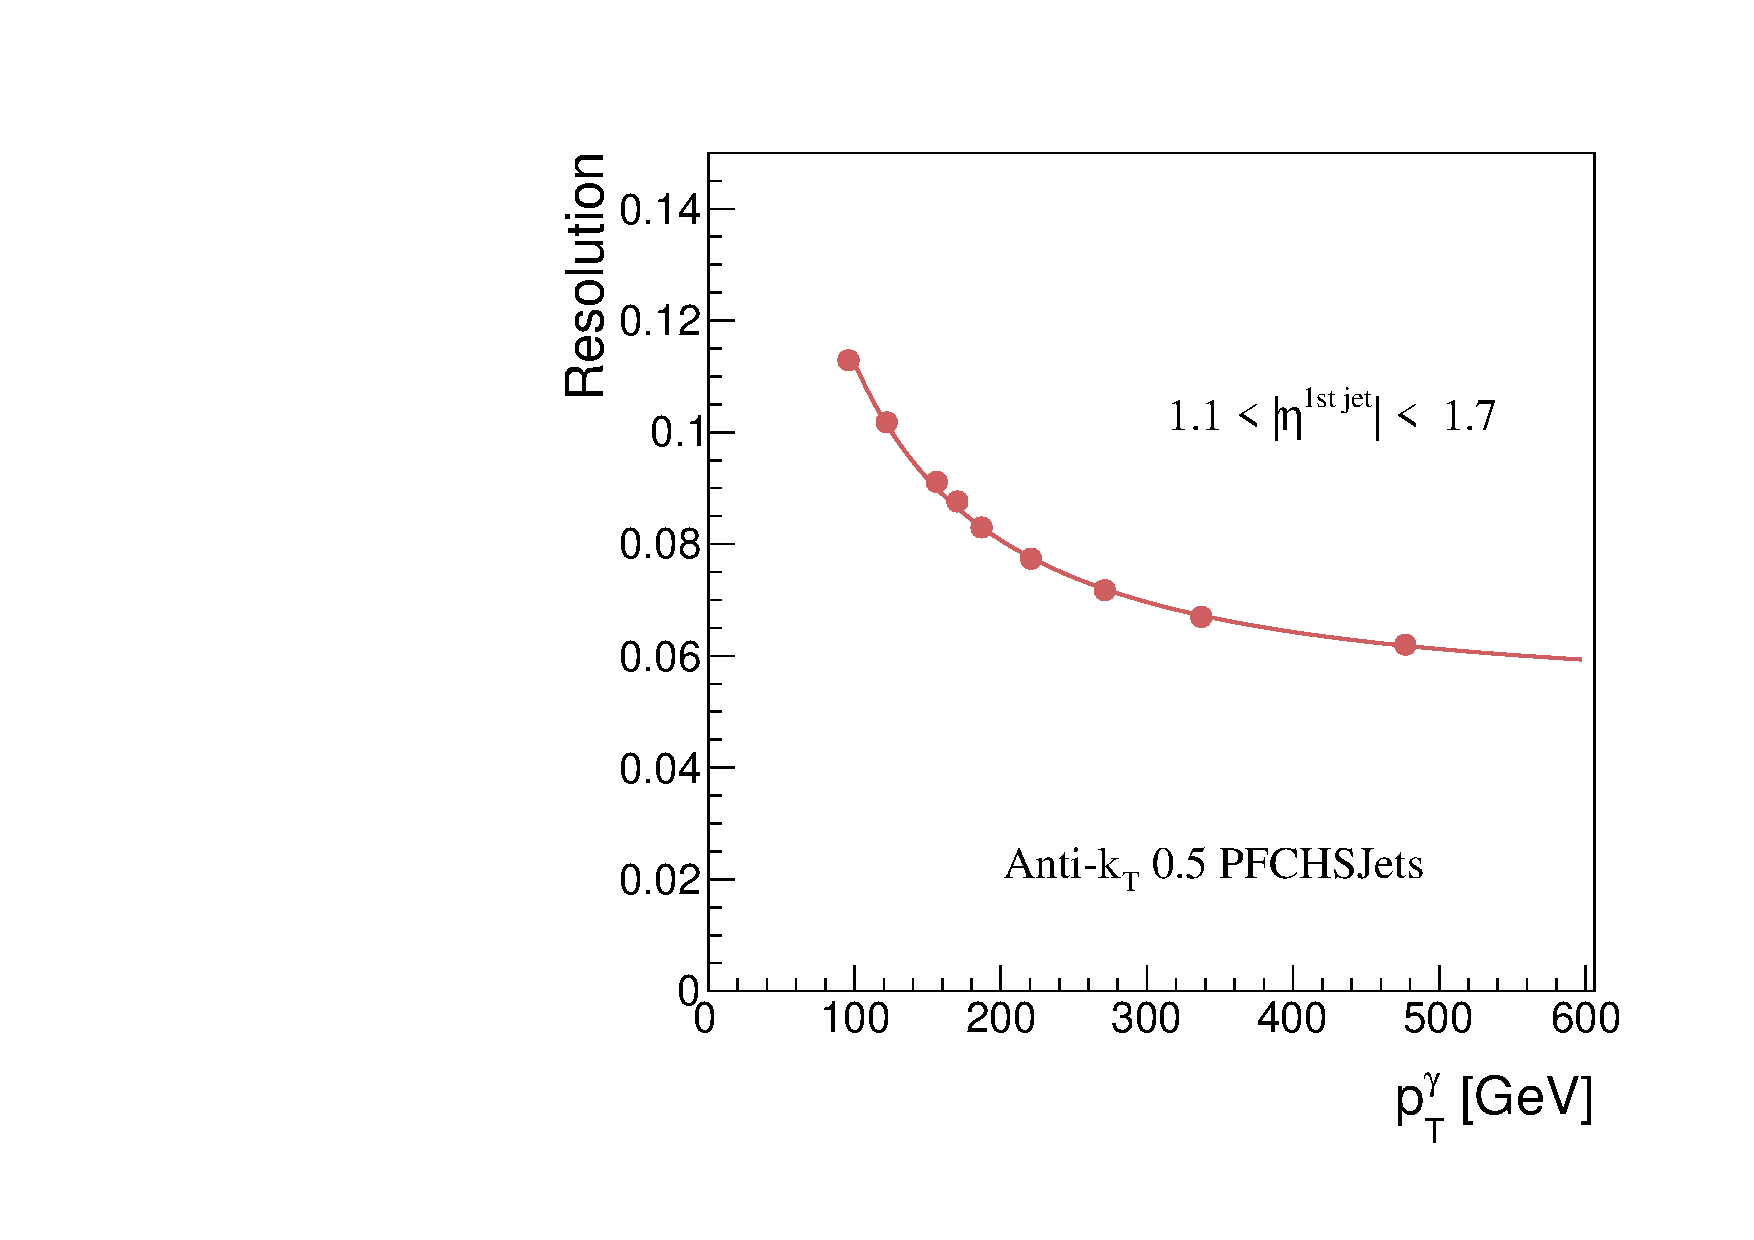
\includegraphics[width=0.49\textwidth]{figures/resolution/methodology/Resolution_for_3_eta_bin_PFCHS_mc_RMS99.pdf}
  \caption{Intrinsic resolution for $|\eta^{\text{1st jet}}| < 0.5$ (left) and $1.1<|\eta^{\text{1st jet}}| < 1.7$ (right) in simulation.}  
  \label{fig:ResolutionOfPtgamma}
\end{figure}
For the $|\eta^{\text{1st jet}}|<0.5$ region, the resolution is approximately 10\% for $\pt^{\gamma} \approx 100\gev$ and decreases to values around 6\% for  
$\pt^{\gamma} \approx 500\gev$.
The increasing statistical uncertainties for low photon \pt arise through the requirement of a maximal $\alpha$ and a minimal \pt of the second jet. 
This reduces the numbers of events in the low photon \pt bins. For events with $\pt^{\gamma}=50\gev$, it is not possible at all to fulfill both requirements at the same time.

The extrapolated intrinsic resolutions for the various photon \pt are fitted with the following function

\begin{equation}
\label{eq:PFresolution}
\text{JER} = \sqrt{\text{sgn(N)} \cdot \frac{\text{N}}{\pt}  + \text{S}^2 \cdot \pt^{\text{M}-1} +  \text{C}^2 }
\end{equation}

which was introduced for particle flow jets in \cite{Chatrchyan:2011ds}. 
It is an extended fit function compared to the usual calorimeter resolution parametrization to account for higher resolution due to tracking information. 

The method is validated with simulated events. 
The bias  is shown in \mbox{Fig. \ref{fig:MCClosure}} for the barrel region. 
\begin{figure}[t]
  \centering

    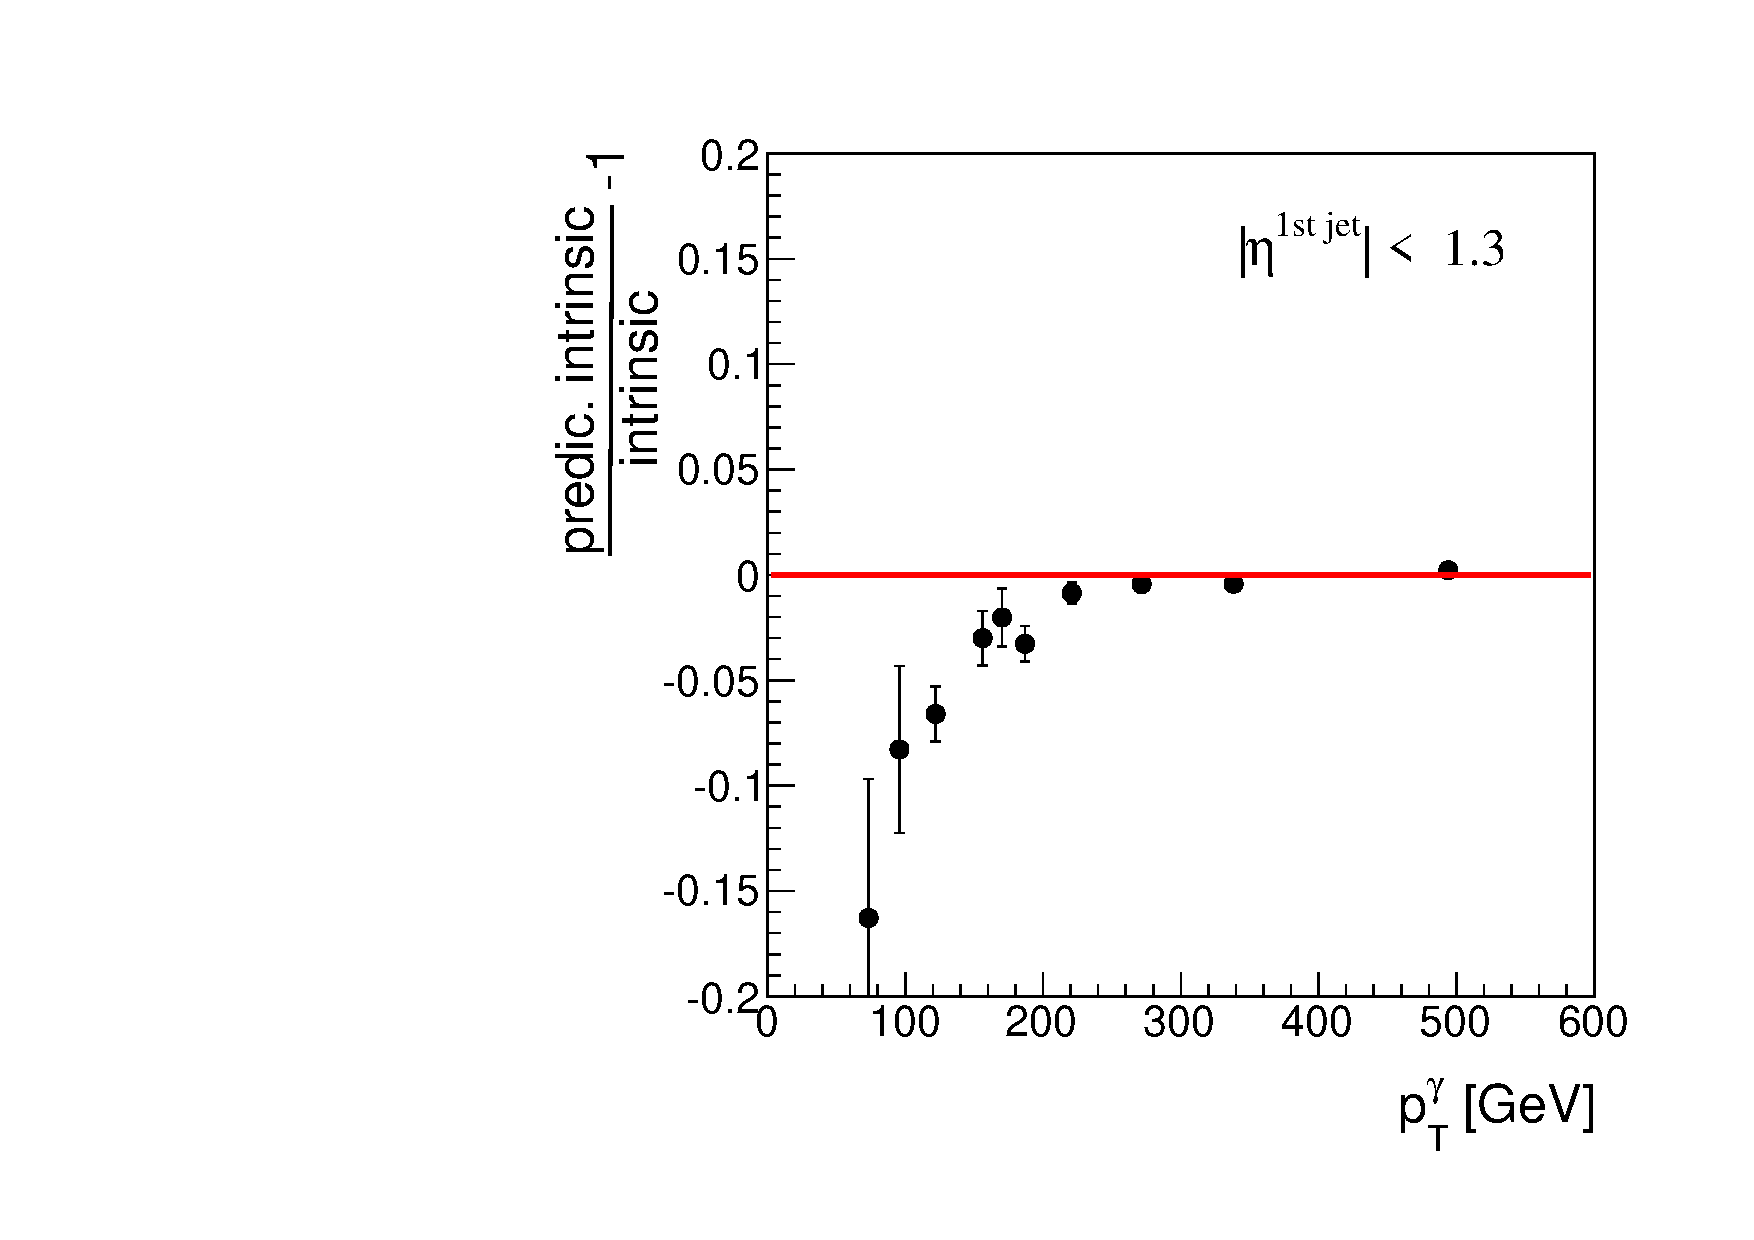
\includegraphics[width=0.49\textwidth]{figures/resolution/methodology/MCClosure_for_1_eta_bin_RMS99_barrel_0p2range.pdf}

  \caption{Consistency check of the method: 
           Comparison between the predicted intrinsic resolution evaluated with \mbox{Eq.~\eqref{eq:total}} 
           and the intrinsic resolution from \mbox{Eq.~\eqref{eq:intrinsic}} in simulation.}  
  \label{fig:MCClosure}
\end{figure}
It is evaluated as the ratio of the predicted intrinsic resolution by fitting \mbox{Eq.~\eqref{eq:total}} with $q^{\prime}$
fixed to the value obtained by \mbox{Eq.~\eqref{eq:imbalance}} over the intrinsic resolution directly obtained from the intrinsic response distribution 
$\frac{\pt^{\text{reco. jet}}}{\pt^{\text{gen. jet}}}$ (MC truth).
The result is in good agreement with the expectation to better than 5\% above $100\gev$ and better than 1\% above $200\gev$.
Only for small \pt, larger deviations are observed, which are systematically lower than zero (up to 15\%).

%The residual bias of the method for small $\pt^{\gamma}$ is originating from the $\alpha$ definition 
%and the decreasing dependence of the resolution on $\pt^{\gamma}$ shown in Figs. \ref{fig:ResolutionOfPtgamma} (a) and (b):\\
%In every $\alpha$ and photon \pt bin, there is a range of various jet \pt.
%Especially for small photon \pt, this leads to differences in the intrinsic resolutions within one $\pt^\gamma$ bin because of the strong $\pt^{\gamma}$ dependence of the resolution.
%Because of the $\alpha$ definition (\mbox{Eq.~\eqref{eq:alphaDef}}) jets with high \pt (and thus better resolution)
%accumulate in the low $\alpha$ bins, whereas jets with low \pt fall in the high $\alpha$ bins. 
%This behavior can be seen in the intrinsic resolution 
%in \mbox{Fig. \ref{fig:AlphaDependenceOfResolutions} \ref{fig:small}}, where a small increase of the resolution to high $\alpha$ can be seen. 
%By fitting a horizontal line to the intrinsic resolution, this effect is averaged out. 
%But the measured resolution with an additional free parameter 
%can adopt this increase and result, therefore, in a y-intercept which is too small. 
%For high photon \pt bins, this effect is less pronounced, as the slope of JER($\pt^{\gamma}$) flattens out.

The residual bias of the method for small $\pt^{\gamma}$ is stemming from two effects: 
First, the binning in $\pt^{\gamma}$ and the momentum balance between the photon and the first two jets 
lead to a dependency of the first jet \pt on the second jet \pt and therefore alpha: 
For a fixed $\pt^{\gamma}$, 
%the greater the second jet pt, the smaller the first jet \pt for events where the second jet is in the leading jet hemisphere 
the \pt of the first jet gets smaller for larger $\pt^{\text{2nd jet}}$ for events where the second jet is in the leading jet hemisphere
(see \mbox{Fig. \ref{fig:sketch}}), leading to a dependency of $\pt^{\text{1st jet}} \propto -\pt^{\text{2nd jet}}$.
This effect is directly opposite for events with a second jet in the photon hemisphere. 
In these events, the first jet \pt gets larger for larger $\pt^{\text{2nd jet}}$ and thus $\pt^{\text{1st jet}} \propto \pt^{\text{2nd jet}}$ for fixed $\pt^{\gamma}$. 
As the resolution of the jet improves with higher jet \pt (see \mbox{Fig. \ref{fig:ResolutionOfPtgamma}}), 
a dependency of the leading jet \pt on the second jet \pt directly leads to a dependency of the intrinsic resolution on the second jet \pt. 
In principle, as the effect is opposite for events in the different hemispheres, it should cancel out, when taking the weighted mean of the two hemisphere resolutions. 
But as the topology of a second jet in the leading jet hemisphere is much more frequent, 
a residual upwards trend in the intrinsic resolution vs. $\alpha$ is conserved. 

The second source of the residual bias arises from the alpha definition $\alpha = \frac{\pt^{\text{2nd jet}}}{\pt^{\gamma}}$. 
Because of the inclusion of $\pt^{\gamma}$ in $\alpha$ with $\alpha \propto \frac{1}{\pt^{\gamma}}$, 
the high photon \pt events accumulate in the low alpha regions. 
As the selected events are almost balanced, a high $\pt^{\gamma}$ is associated with a high jet \pt, thus also the high jet \pt events accumulate in the low alpha bins, 
leading to  an upward trend in the intrinsic resolution. This behavior can be seen in the intrinsic resolution 
in Fig.~\ref{fig:AlphaDependenceOfResolutions}, where a small increase of the resolution to high $\alpha$ can be seen. 
By fitting a horizontal line to the intrinsic resolution, this effect is averaged out. 
But the measured resolution with an additional free parameter 
can adopt this increase and result, therefore, in a y-intercept which is too small. 
For high photon \pt bins, this effect is less pronounced, as the slope of JER($\pt^{\gamma}$) (see Fig.~\ref{fig:AlphaDependenceOfResolutions}) flattens out.

However, this is not of concern here, because the results of the measurement will be presented as resolution scaling factors, defined as the resolution measured in data divided by
the resolution measured in Monte Carlo simulation (MC) $\frac{\text{JER}^{\text{data}}}{\text{JER}^{\text{MC}}}$. 
Hence, a possible bias in the separate resolution measurements for data and simulation cancels out. 

As the data to simulation ratio was empirically found to be independent of $\pt^{\gamma}$, it can be fitted with a constant.
Thus resulting in only one scaling factor for every $\eta^{\text{1st jet}}$ region.


To prove the hypothesis of the cancellation of the bias, the data set with simulated 
events was additionally smeared with some input values for various $\eta^{\text{1st jet}}$ bins. 
After measuring the resolution of the smeared and non-smeared data set, the relative difference between the two data sets  
($\frac{\text{JER}_{\text{smeared MC}}}{\text{JER}_{\text{non-smeared MC}}}$) is fitted with a constant over the photon \pt range. 
The resulting numbers (one for each $\eta^{\text{1st jet}}$ bin) are then compared to the input factors. 

In \mbox{Fig. \ref{fig:MCClosureRatio}}, a comparison of the input and output values is shown. The resolution is hereby defined in three different ways: 
The standard deviations of the 99\% and 95\% truncated response distribution and as the width of a Gaussian 
\footnote{The Gaussian width is defined as the standard deviation of the 2$\sigma$ interval (core region) around the mean, where the determination of $\mu$ and $\sigma$ were approximated with an iterative procedure.}.

\begin{figure}[tbp]
  \centering

    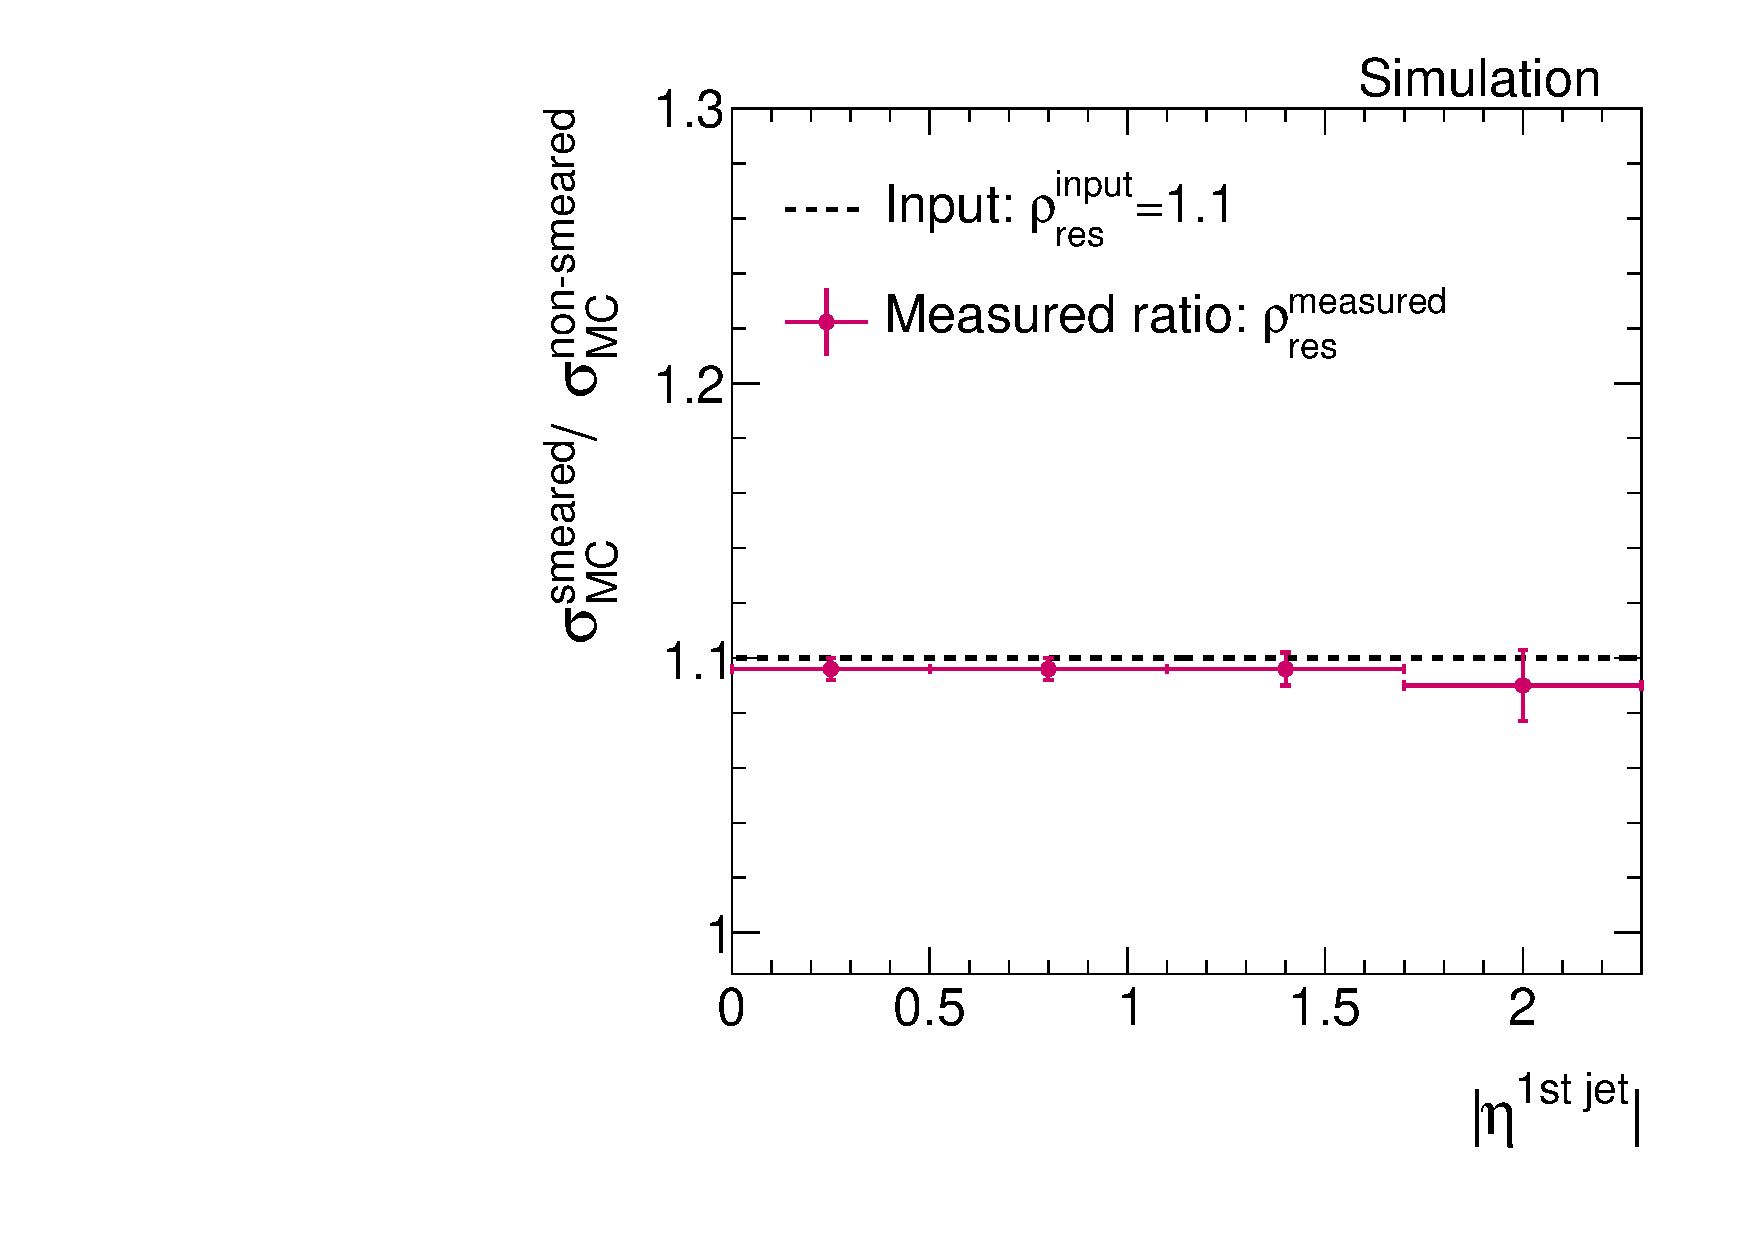
\includegraphics[width=0.49\textwidth]{figures/resolution/methodology/MCClosureRatio.pdf}

  \caption{Comparison of the resolution ratios $\frac{\text{JER}_{\text{smeared MC}}}{\text{JER}_{\text{non-smeared MC}}}$ 
           measured in simulated events with the input smearing factors 1.05, 1.07, 1.09 and 1.11 (black dots) for the various $\eta^{\text{1st jet}}$ bins, respectively. 
           Shown are the results for a Gaussian fit of the response 
           distribution (blue triangles), a standard deviation of the 99\% (red squares) and the 95\% truncated response (green dots).}
  \label{fig:MCClosureRatio}
\end{figure}

In all cases, the measurement reproduces the input factors.
However, in this analysis the 99\% truncated response will be used to be consistent with the defintion from \cite{CMS-AN-2010-076}.

In the following section, the systematic uncertainties will be discussed. Afterward, results will be presented.


%%%%%%%%%%%%%%%%%%%%%%%%%%%%%%%%%%%%%%%%%%%%%%%%%%%%%%%%%%%%%%%%%%%%%%%%%%%%%%%%%%%%%%%%%%%%%%%%%%%%%%%%%%%%%%%%%%%%%%%%%%%%%%%%%%%%%%%%%%%%%%%%%%%%%%%%%%%%%%%%%%%%%%%%%%%%%%%%%%%%%%%%%%%%%%%%%%%%%%%%%%%%%%%%%%%%%%%%%%%%%%%%%%%%%%%%%%%

%%%%%%%%%%%%%%%%%%%%%%%%%%%%%%%%%%%%%%%%%%%%%%%%%%%%%%%%%%%%%%%%%%%%%%%%%%%%%%%%%%%%%%%%%%%%%%%%%%%%%%%%%%%%%%%%%%%%%%%%%%%%%%%%%%%%%%%%%%%%%%%%%%%%%%%%%%%%%%%%%%%%%%%%%%%%%%%%%%%%%%%%%%%%%%%%%%%%%%%%%%%%%%%%%%%%%%%%%%%%%%%%%%%%%%%%%%%
%%%%%%%%%%%%%%%%%%%%%%%%%%%%%%%%%%%%%%%%%%%%%%%%%%%%%%%%%%%%%%%%%%%%%%%%%%%%%%%%%%%%%%%%%%%%%%%%%%%%%%%%%%%%%%%%%%%%%%%%%%%%%%%%%%%%%%%%%%%%%%%%%%%%%%%%%%%%%%%%%%%%%%%%%%%%%%%%%%%%%%%%%%%%%%%%%%%%%%%%%%%%%%%%%%%%%%%%%%%%%%%%%%%%%%%%%%%
\chapter{Systematic uncertainties}

\begin{itemize}
\item difficult to take from AN
\end{itemize}

Pictures as root file available:
\begin{itemize}
\item BLA
\end{itemize}

Picture \textcolor{red}{NOT} as root file available:
\begin{itemize}
\item BLA
\end{itemize}
%%%%%%%%%%%%%%%%%%%%%%%%%%%%%%%%%%%%%%%%%%%%%%%%%%%%%%%%%%%%%%%%%%%%%%%%%%%%%%%%%%%%%%%%%%%%%%%%%%%%%%%%%%%%%%%%%%%%%%%%%%%%%%%%%%%%%%%%%%%%%%%%%%%%%%%%%%%%%%%%%%%%%%%%%%%%%%%%%%%%%%%%%%%%%%%%%%%%%%%%%%%%%%%%%%%%%%%%%%%%%%%%%%%%%%%%%%%

%%%%%%%%%%%%%%%%%%%%%%%%%%%%%%%%%%%%%%%%%%%%%%%%%%%%%%%%%%%%%%%%%%%%%%%%%%%%%%%%%%%%%%%%%%%%%%%%%%%%%%%%%%%%%%%%%%%%%%%%%%%%%%%%%%%%%%%%%%%%%%%%%%%%%%%%%%%%%%%%%%%%%%%%%%%%%%%%%%%%%%%%%%%%%%%%%%%%%%%%%%%%%%%%%%%%%%%%%%%%%%%%%%%%%%%%%%%
%%%%%%%%%%%%%%%%%%%%%%%%%%%%%%%%%%%%%%%%%%%%%%%%%%%%%%%%%%%%%%%%%%%%%%%%%%%%%%%%%%%%%%%%%%%%%%%%%%%%%%%%%%%%%%%%%%%%%%%%%%%%%%%%%%%%%%%%%%%%%%%%%%%%%%%%%%%%%%%%%%%%%%%%%%%%%%%%%%%%%%%%%%%%%%%%%%%%%%%%%%%%%%%%%%%%%%%%%%%%%%%%%%%%%%%%%%%
\chapter{Results}

\begin{itemize}
\item THINK
\end{itemize}

Pictures as root file available:
\begin{itemize}
\item BLA
\end{itemize}

Picture \textcolor{red}{NOT} as root file available:
\begin{itemize}
\item BLA
\end{itemize}
%%%%%%%%%%%%%%%%%%%%%%%%%%%%%%%%%%%%%%%%%%%%%%%%%%%%%%%%%%%%%%%%%%%%%%%%%%%%%%%%%%%%%%%%%%%%%%%%%%%%%%%%%%%%%%%%%%%%%%%%%%%%%%%%%%%%%%%%%%%%%%%%%%%%%%%%%%%%%%%%%%%%%%%%%%%%%%%%%%%%%%%%%%%%%%%%%%%%%%%%%%%%%%%%%%%%%%%%%%%%%%%%%%%%%%%%%%%

%%%%%%%%%%%%%%%%%%%%%%%%%%%%%%%%%%%%%%%%%%%%%%%%%%%%%%%%%%%%%%%%%%%%%%%%%%%%%%%%%%%%%%%%%%%%%%%%%%%%%%%%%%%%%%%%%%%%%%%%%%%%%%%%%%%%%%%%%%%%%%%%%%%%%%%%%%%%%%%%%%%%%%%%%%%%%%%%%%%%%%%%%%%%%%%%%%%%%%%%%%%%%%%%%%%%%%%%%%%%%%%%%%%%%%%%%%%
%%%%%%%%%%%%%%%%%%%%%%%%%%%%%%%%%%%%%%%%%%%%%%%%%%%%%%%%%%%%%%%%%%%%%%%%%%%%%%%%%%%%%%%%%%%%%%%%%%%%%%%%%%%%%%%%%%%%%%%%%%%%%%%%%%%%%%%%%%%%%%%%%%%%%%%%%%%%%%%%%%%%%%%%%%%%%%%%%%%%%%%%%%%%%%%%%%%%%%%%%%%%%%%%%%%%%%%%%%%%%%%%%%%%%%%%%%%
\chapter{Discussion and conclusion}

\begin{itemize}
\item Repeat results
\item cross-check analysis
\item Outlook
\end{itemize}

Pictures as root file available:
\begin{itemize}
\item BLA
\end{itemize}

Picture \textcolor{red}{NOT} as root file available:
\begin{itemize}
\item BLA
\end{itemize}
